\documentclass[12pt,a4paper]{report}
\usepackage[margin=2.5cm]{geometry}
\usepackage[magyar]{babel}

% magyar nyelv tamogatas
\usepackage{t1enc}
\usepackage[T1]{fontenc}
\usepackage[utf8]{inputenc}

% A formai kovetelmenyekben megkövetelt Times betűtípus hasznalata:
\usepackage{times}

\usepackage{setspace}
\usepackage{listings,multicol}
\usepackage{xcolor}
\usepackage{textcomp}
\usepackage{enumitem}
\usepackage{booktabs}
\usepackage[unicode,hidelinks]{hyperref}
\usepackage{footnote}
\usepackage{ifthen}

% Törölhető package
\usepackage{lipsum}

% TODO csomag, amivel jól észrevehető todokat hagyhatunk a dolgozatban
\usepackage{todonotes}
% Inline TODO
\newcommand{\todoi}[1]{\todo[inline]{\textbf{TODO:} #1}}

% egyedi lablec
\usepackage{fancyhdr}
\renewcommand{\headrulewidth}{0.0pt}% Default \headrulewidth is 0.4pt

\usepackage{graphicx}
\graphicspath{{fig/}}

% Kódrészletes színezése
\definecolor{listinggray}{gray}{0.9}
\definecolor{lbcolor}{rgb}{0.9,0.9,0.9}
\lstset{
 language=Bash,
 keywordstyle=\bfseries\ttfamily\color[rgb]{0,0,1},
 identifierstyle=\ttfamily,
 commentstyle=\color[rgb]{0.133,0.545,0.133},
 stringstyle=\ttfamily\color[rgb]{0.627,0.126,0.941},
 showstringspaces=false,
 basicstyle=\scriptsize,
 numberstyle=\tiny,
 numbers=none,
 stepnumber=1,
 numbersep=10pt,
 tabsize=2,
 breaklines=true,
 prebreak = \raisebox{0ex}[0ex][0ex]{\ensuremath{\hookleftarrow}},
 breakatwhitespace=false,
 aboveskip={0.5\baselineskip},
 columns=fixed,
 upquote=true,
 extendedchars=true,
 frame=single,
 backgroundcolor=\color{lbcolor},
 literate={`}{\textasciigrave}{1}
}


\definecolor{sajatzold}{RGB}{0,105,0}

\lstdefinelanguage{diff}{
  morecomment=[f][\color{blue}]{@@},     % group identifier
  morecomment=[f][\color{red}]-,         % deleted lines
  morecomment=[f][\color{sajatzold}]+,       % added lines
  morecomment=[f][\color{magenta}]{---}, % Diff header lines (must appear after +,-)
  morecomment=[f][\color{magenta}]{+++},
}

\renewcommand{\lstlistingname}{Kódrészlet}

% Margók beállítása
\hoffset -1in
\voffset -1in
\oddsidemargin 35mm
\textwidth 150mm
\topmargin 15mm
\headheight 10mm
\headsep 5mm
\textheight 237mm

% Szerző és dolgozat adatai
%Szerző adatai
\newcommand{\nev}{Sándor Márton}
\newcommand{\szak}{programtervező informatikus BSc}
\newcommand{\tanszek}{Szoftverfejlesztés}
\newcommand{\ev}{2025}
\newcommand{\dolgozatTipusa}{Szakdolgozat}
%\newcommand{\dolgozatTipusa}{Diplomamunka}
\newcommand{\vegsoDatum}{\today}

\newcommand{\cim}{Fogászati rendelő webalkalmazás implementálása Django keretrendszerben}

%Témavezető adatai
\newcommand{\temavezetoNev}{Antal Gábor}
\newcommand{\temavezetoBeosztas}{egyetemi docens}


\begin{document}

% Másfeles sorköz
\setstretch{1.5}
\sloppy

\thispagestyle{fancy}
% A címoldalra se fej- se lábléc nem kell:
% \thispagestyle{empty}
\pagenumbering{gobble}
\begin{center}
  \vspace*{0.5cm}
  {
    \Large\bf Szegedi Tudományegyetem}

    \vspace{0.1cm}

    {\Large\bf Informatikai Intézet}

    \vspace*{4.2cm}


    {\LARGE\bf \cim}


    \vspace*{3.4cm}

    {\Large \dolgozatTipusa}

    \vspace*{3.5cm}

    %Értelemszerűen megváltoztatandó:
    {\large
    \noindent
    \begin{tabular}{@{}c@{\hspace{1cm}}c}
    \emph{Készítette:}     & \emph{Témavezető:}\\
    \bf{\nev}              & \bf{\temavezetoNev}\\
    \szak                  & \temavezetoBeosztas\\
    szakos hallgató        &
    \end{tabular}
    }

    \vspace*{2.3cm}

    {\Large
    Szeged
    \\
    \vspace{2mm}
    \ev
  }
\end{center}

\pagenumbering{arabic}
\chapter*{Feladatkiírás}
\addcontentsline{toc}{section}{Feladatkiírás}
A szakdolgozat célja, hogy a hallgató megismerkedjen az egyik legismertebb Python alapú webes keretrendszerrel, a Django-val. A megszerzett ismeretei segítségével a hallgató egy fogászati szakrendelőnek tervezett időpontfoglalási rendszert épít, amelyben elérhető a PayPal fiókos, és a bankkártyás fizetés, és az időpontfoglalás. A rendelő orvosainak lehetőségük van a saját munkaidejük bevitelére, a páciensek kezeléstörténetének megtekintésére, és a magukhoz foglalt időpontok megtekintésére. Továbbá bármelyik páciens adatait és elérhetőségeit megtekinthetik. A rendszer emellett küld emailes értesítéseket is, hogy a felhasználók és az orvosok is kapjanak információkat a foglalásokról. Az alkalmazás tartalmaz admin felületet is, amivel a felhasználónak joga van új orvosokat hozzáadni a rendszerhez, a felhasználóknak új jelszót adni, és az adatbázisban tárolt kezeléseket létrehozni, szerkeszteni, vagy törölni. A felhasznált adatbázis kezelő rendszer a Django beépített rendszere, ami sqlite3 adatbázist használ.
\lipsum[3-5]
\chapter*{Tartalmi összefoglaló}
\addcontentsline{toc}{section}{Tartalmi összefoglaló}

\noindent\textbf{A téma megnevezése:}

\noindent Fogászati rendelő webalkalmazás implementálása Django keretrendszerben

\noindent\textbf{A megadott feladat megfogalmazása:}

\noindent A Django keretrendszer által nyújtott előnyök megismerése, felhasználása a fogászati rendelő időpontfoglalási rendszerének fejlesztéséhez. Az alkalmazásnak rendelkeznie kell felhasználói, orvosi, és adminisztrátori felülettel. Meg kell valósítani az online időpontfoglalás, és az online fizetés lehetőségét. Az orvosoknak meg kell valósítani egy felületet amivel vissza tudják nézni a páciens kezeléstörténetét. Az adatokat pedig FHIR szabvány szerint kell tárolni, hogy bármilyen más egészségügyi rendszerrel kompatibilis legyen.

\noindent\textbf{A megoldási mód:}

\noindent Megismerkedtem a Django keretrendszerrel, annak felépítésével. Megterveztem a rendelő webalkalmazásának adatbázis-struktúráját, amely tartalmazza a páciensek, orvosok, kezelések és időpontfoglalások moduljait. Az alkalmazás reszponszív felhasználói felületét modern CSS megoldásokkal építettem ki, míg a backend részben a Django admin és REST API-k biztosítják az adatok hatékony kezelését. Emellett integráltam a PayPal fizetési rendszert az online fizetések lebonyolításához. A fejlesztés során a projektet GitHubon verzióztam, biztosítva ezzel a kód stabilitását és könnyű karbantarthatóságát.

\noindent\textbf{Alkalmazott eszközök, módszerek:}

\noindent Git, Github, Django, SQLite, HTML, JavaScript, CSS, Python

\noindent\textbf{Elért eredmények:}

\noindent Megismertem a Djangot, és az általa nyújtott lehetőségeket, a PayPal integrációt, a Python nyelvet, az FHIR szabványt, és a webfejlesztést. Sikeresen működik az általam integrált időpontfoglalási és fizetési rendszer.

\noindent\textbf{Kulcsszavak:}

\noindent Django, SQLite, HTML, JavaScript, CSS, Python, ORM

\addcontentsline{toc}{section}{Tartalomjegyzék}

\thispagestyle{plain}
\tableofcontents
\setlength{\parindent}{0pt}


\pagestyle{fancy}
\fancyhf{}
\fancyhead[L]{\textit{\cim}}
\fancyfoot[R]{\thepage}
\renewcommand{\headrulewidth}{0.4pt}% Default \headrulewidth is 0.4pt

\chapter{A Django keretrendszer}
\label{chap:intro}

A Django egy magas szintű Python webkeretrendszer, amely támogatja a gyors fejlesztést és az egyszerű, jól átgondolt megoldásokat. Tapasztalt fejlesztők által készített, így számos webfejlesztési nehézséget megold, és lehetővé teszi, hogy a fejlesztő alkalmazás írására koncentráljon, anélkül, hogy újra fel kellene találnia a kereket. További pozitívuma, hogy ingyenes, és nyílt forráskódú.\cite{Djangoproject}

\section{Az MVT programszervezési minta}

Django projekt lévén az alkalmazás az MVT (Model View Template) design pattern alapelveit kell, hogy kövesse. Ez áll a model-ből, ahol az adatbázis struktúrájáját építjük fel, a view-ból, ami lényegében a projekt azon része, ahol a háttérfolyamatok futnak, és a template-ből, ami a felhasználói felületet tartalmazza. Ez a kapcsolata a felhasználónak az alkalmazással.

\section{Model}

A Model-ek a Django alkalmazáson belüli adatszerkezet kezelését és interakcióját irányítják, így a Django alkalmazások alapját képezik, mivel az adatok kritikus szerepet játszanak.
A Django Model-ek egy erőteljes, Objektum-Relációs Leképezést (ORM: Object-Relational Mapping) megvalósító funkciót használnak, amely áthidalja a szakadékot a relációs adatbázis és a Python kód között. Ez a leképezés a Python objektumokat (osztályokat) adatbázis táblákká alakítja, az osztályok attribútumait oszlopokká, és az egyes példányokat a táblák soraivá.
Az ORM egyik nagy előnye, hogy lehetővé teszi az adatbázissal való interakciót Python objektumokon keresztül, anélkül, hogy SQL lekérdezéseket kellene írnunk.
A Django Model-ek összegzik az összes adatbázissal kapcsolatos logikát és meghatározzák az adatbázis szerkezetét, mint egy tervrajzot annak, hogy milyen adatokat szeretnénk tárolni.\cite{MVT_Design}

\section{View}

Ha az MVC modellhez szeretnénk hasonlítani, akkor az MVT modellben a View hasonló, mint az MVC-ben a Controller.
A Django view-k felelősek a felhasználói kérések feldolgozásáért és a válaszok visszaküldéséért. Híd szerepét töltik be a Model és a Template között: Adatokat gyűjtenek a Model-ből, logikai műveleteket (például bizonyos kritériumok alapján végzett lekérdezéseket) hajtanak végre rajtuk, majd az eredményeket átadják a Template-nek a megjelenítéshez.
A View-kat függvényekként vagy osztály alapú View-ként is megírhatjuk, attól függően, hogy az alkalmazásunk komplexitása és követelményei melyik megközelítést igénylik.\cite{MVT_Design}

\section{Template}

A Django Template-ek feladata, hogy a böngészőben megjelenítendő végső HTML kimenetet rendereljék. Meghatározzák, miként kell az adatokat bemutatni, HTML és a Django sablonnyelvének kombinációjával.
A Django sablonnyelv template tageket \verb|()| és template változókat \verb|({{ }})| alkalmaz, amelyek lehetővé teszik, hogy a sablon HTML kódjában Django módba lépjen, és így hozzáférjen a View-kban definiált változókhoz, illetve vezérlési struktúrákat használjon a megjelenítés szabályozására.
A sablonok továbbá formázhatók CSS-sel, illetve bármely kedvelt CSS keretrendszerrel, hogy a felhasználói felület mégszebb legyen. Emellett animálhatók is JS segítségével.\cite{MVT_Design}





\chapter{Alkalmazás struktúrája}
\label{chap:fejezet2}

Egy Django projekt esetében a projekt felépítése modulárisan, egy vagy több alkalmazásból (app) áll, melyek mindegyike egy adott funkcionális területért felel. A szakdolgozatom esetében a "rendelo" mappa tartalmazza a teljes webalkalmazás forráskódját.\\
A "rendelo" mappa a következő részekből áll:

\begin{itemize}
	\item Gyökérszint:
	\begin{itemize}
		\item manage.py: A Django projekt parancssori kezelője, amely a fejlesztési feladatok (például migrációk futtatása, szerver indítása) végrehajtását segíti.
		\item db.sqlite3: Az alapértelmezett, fejlesztési környezetben használt SQLite adatbázis fájlja.
	\end{itemize}
	\item Projekt főkönyvtára ("rendelo"): Itt találhatók a projekt globális beállításait és konfigurációs fájljait, mint például a settings.py, urls.py, wsgi.py és asgi.py. Ezek a fájlok felelősek az alkalmazás működésének alapvető paramétereinek meghatározásáért, az útvonalak kezeléséért és a szerverrel való kommunikációért.
	\item Alkalmazás könyvtára ("rendeloweboldal"): Ez a rész tartalmazza a rendszer egyes moduljait, amelyek a következő fő komponensekből állnak:
	\begin{itemize}
		\item models.py: Az adatbázis szerkezetét definiáló modellek, melyek meghatározzák a páciensek, orvosok, kezelések, időpontfoglalások és az időpont foglalások fizetési státuszának struktúráját.
		\item views.py: A felhasználói kérések feldolgozásáért és az üzleti logika megvalósításáért felelős fájl, amely összeköti a modelleket a sablonokkal.
		\item forms.py: Az űrlapok és azok validációs szabályainak definíciója, melyek révén az adatbevitel és ellenőrzés történik.
		\item urls.py: Az alkalmazás specifikus URL-konfigurációja, amely a különböző view-k elérését biztosítja.
		\item admin.py: A Django beépített adminisztrátori felület konfigurációját tartalmazza. Hozzá kell adni az összes modellt az adatbázisból, amit elérhetővé szeretnénk tenni rajta.
		\item migrations/: Az adatbázis változásait követő migrációs fájlokat tartalmazza, dokumentálva a modellek módosításait.
		\item static/ és templates/: A statikus fájlokat (CSS, JavaScript, és az alkalmazás designjához tartozó képek) illetve a HTML template-eket rendszerezi, amelyek a felhasználói felület megjelenítéséért felelősek.
	\end{itemize}
\end{itemize}

A projekt kialakítása moduláris és átlátható, mely lehetővé teszi a fejlesztés, karbantartás és bővítés egyszerű kezelését.
Emellett a projekt verziókezelése a GitHubon történik, így könnyen nyomon követhető az egész alkalmazás fejlesztése.
\chapter{Adatbázis}
\label{chap:fejezet3}

\section{Az adatbázis típusa}
Először is el kell döntenünk, hogy milyen adatbázist fogunk használni a fejleszteni kívánt alkalmazásunkhoz. Ennek sok szempontja lehet, például hogy mekkora mennyiségű adattal szeretnénk dolgozni, vagy hogy mennyire kell gyorsnak lennie a lekérdezéseknek.

\begin{figure}[!htbp]
	\caption{Példa az adatbázis beállításra}
	\label{fig:adatbazisbeallitas}
	\centering
	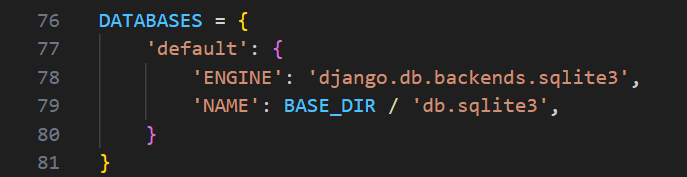
\includegraphics[width=1.0\textwidth]{database_setting.png}
\end{figure}

A szakdolgozatomban a Django beépített adatbázisát használtam, ami sqlite3, mivel egy fogászati rendelőnek nincsen nagyon nagy adatforgalma, így elegendő hozzá ez a fajta adatbázis. A 3.1 ábrán látható egy példa az adatbázis típusának beállítására. Ezt a beállítást a settings.py fájlban kell megadni, ami az én alkalmazásomban a projekt fő mappáján belüli "rendelo" nevú mappában található.

\section{Az adatbázis felépítése}
Az adatbázis típusának kiválasztása után a legfontosabb rész következik: Felépíteni az adatbázis szerkezetét. Mivel ORM technológiát használ a keretrendszerünk így szerencsére nincs szükségünk SQL ismeretekre ennek a műveletnek a végrehajtásához. Django-ban minden alkalmazásnak van egy (vagy több) models.py nevű fájlja. Ebbe importálnunk kell a Django models modulját, amit így tehetünk meg:\\
from django.db import models\\
Ezután python osztályként beleírhatjuk a fájlba a tárolni kívánt adatok tulajdonságait. Az ORM-ben az adatbázis táblák oszlopait a python osztályaink adják meg, és az adatbázis rekordok ezeknek a példányaiból keletkeznek. Minden model osztálynak közvetlenül, vagy közvetetten a models.Model modulból kell származnia. A nem közvetlen származás a python nyelv többszörös öröklődés támogatása miatt lehetséges.

\begin{figure}[!htbp]
	\caption{Példa az adatbázis model leírására}
	\label{fig:adatbazismodell}
	\centering
	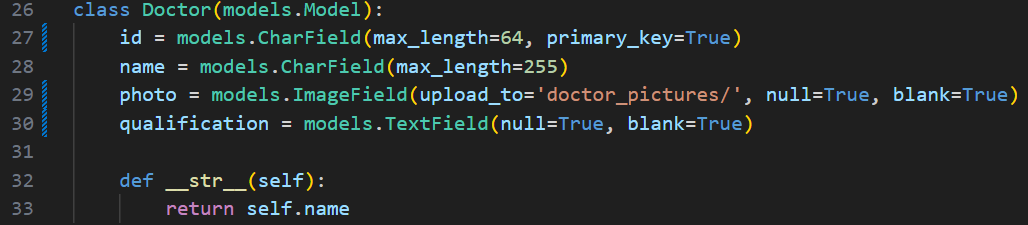
\includegraphics[width=1.0\textwidth]{database_model_example.png}
\end{figure}

A szakdolgozatomban egyértelmű volt, hogy FHIR szabványú adatbázissal kell dolgoznom, mivel az egészségügyi alkalmazásoknak ez a szabványa. Azért éri meg így kialakítani az adatbázist, mert ezzel a módszerrel az összes egészségügyi rendszerrel kompatibilis rendszert hozhatunk létre. A 3.2. ábrán látható az egyik FHIR szabványú model osztály a szakdolgozatomból.\\
A model-ek megírása nem volt egyszerű, mivel meg kellett oldanom a profilkezelést és az autentikációt az alkalmazásban, viszont szabványosnak kellett maradnia. Ezzel az a probléma, hogy az FHIR szabvány nem támogat profilkezelést.\\
Az alkalmazás model osztályai:
\begin{itemize}
	\item RendeloUser
	\item Patient
	\item Doctor
	\item Treatment
	\item Appointment
	\item WorkingHours
	\item PaymentStatus
\end{itemize}

\subsection{Profilkezelés}

\begin{figure}[!htbp]
	\caption{A felhasználói profilokat tároló model}
	\label{fig:profilmodell}
	\centering
	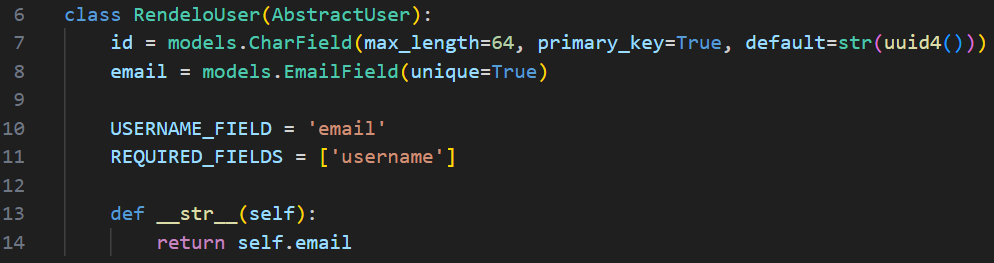
\includegraphics[width=1.0\textwidth]{abstractuser_model.png}
\end{figure}

Az alkalmazásomban három felhasználói jogosultságú profil elérhető:

\begin{itemize}
	\item Superuser: Adminisztrátor akinek mindenhez van joga, bármilyen adatot törölhet, meg van valósítva a számára egy külön "Admin" nevű oldal amin az adatok kezeléséhez hozzáfér, és beléphet a Django beépített adminisztrátori felületére is.
	\item Staff: A fogászati rendelő orvosainak a jogosultságával rendelkezik. Ezeket a profilokat az adminisztrátor tudja létrehozni az "Admin" oldalon. Minden ilyen profil megjelenik orvosként az orvosok kiválasztásánál az időpontfoglalás során. Joga van megtekinteni a páciensek kezeléstörténetét, és szerkeszteni azt. Joga van az összes hozzá foglalt időpont megtekintésére, a páciensek adatainak lekérdezésére, és a saját munkaidejének a beállítására.
	\item User: A páciensek felhasználói fiókjai, a Regisztrációs oldalon hozhatók létre. Az időpontfoglaláshoz csak ezeknek a fiókoknak van joga, emellett megtekinthetik a saját kezeléstörténetüket és az időpontjaikat, illetve le is mondhatják azokat.
\end{itemize}

A profilokat a 3.3. ábrán látható RendeloUser osztály tárolja. Az osztály az AbstractUser-ből származik, ami a Django beépített autentikációs rendszerébe tartozik. Amikor létrehozunk az alkalmazásban egy bármilyen jogosultsággal rendelkező profilt, akkor ez az osztály fogja tárolni a bejelentkezéshez szükséges adatainkat. Superuser esetén csak ez az egy objektum tartozik a profilunkhoz, mivel az adminisztrátor nem orvos, és nem páciens, nincs szüksége további adat tárolására.\\

Ha az adminisztrátor létrehoz egy új orvosnak egy profilt az alkalmazásban, akkor először is létrejön a RendeloUser példány, amihez generálódik egy uuid4 egyedi azonosító, ami $id$ néven van tárolva a 3.3. ábrán látható módon. Ezután létrejön egy FHIR szabványos Doctor osztálypéldány is, ami az orvos adatait tárolja. Ennek az osztálynak is van egy $id$ nevű, karaktersorozat típusú adattagja, amibe bemásolja a program a RendeloUser objektumban létrehozott egyedi azonosítót. Így kapcsolódik össze a két osztálypéldány. Ezen kívül a program hozzáadja a többi tárolni kívánt adatát az orvosnak.\\

Hasonló folyamat történik, amikor egy user szintű felhasználó regisztrál az akalmazásba. Először létrejön a RendeloUser példány az egyedi uuid4 azonosítóval, ezután létrejön egy FHIR szabványos Patient objektum, amiben a páciens adatait tároljuk, a Patient objektum $id$ nevú karaktersorozat típusú adattagjába pedig bemásolja a program az egyedi azonosítót, így összekapcsolta a profiladatokat tároló RendeloUser példányt a páciens adatokat tároló Patient példánnyal. Ezek után pedig elmenti a user további adatait is. A 3.4. ábrán látható a Patient model.

\begin{figure}[!htbp]
	\caption{A Patient model}
	\label{fig:patientmodel}
	\centering
	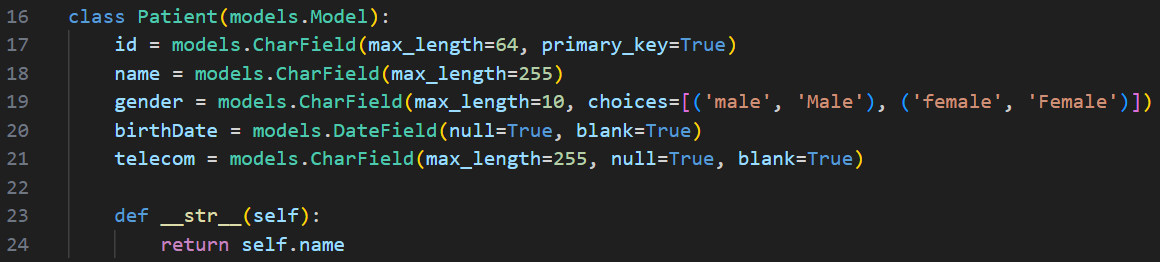
\includegraphics[width=1.0\textwidth]{patient_model.png}
\end{figure}

\subsection{Az időpontfoglalás adatainak tárolása}

Az időpontfoglalás adatait három model-ben tárolja az alkalmazás:

\begin{itemize}
	\item Treatment model: A kezelés típusát tárolja, amire időpontokat lehet foglalni. A kezeléseket az adminisztrátor viszi fel az adatbázisba. A Treatment-nek is van egy $id$ adattagja amibe generálódik automatikusan az uuid4, ezen kívül tárol egy nevet, leírást, egy hosszt, ami azt tárolja, hogy mennyi ideig tart, illetve egy árat ami forintban értendő. Ez a model is FHIR szabványt követ.
	\item Appointment model: A lefoglalt időpontot tárolja. Ez az osztálypéldány a páciensek időpontfoglalásának a hatására jön létre. Tárolja a saját id-ját ami automatikusan generálódik a számára amikor létrejön, ezen kvívül van egy $patient$ adattagja ami az időpontot lefoglaló páciens id-ját tárolja. A $practitioner$ adattag ahhoz az orvoshoz kapcsolódik ForeignKey-ként, akihez a páciens időpontot foglalt. Erre azért volt szükség, hogy ha töröljük az orvost az adatbázisból, akkor a hozzá foglalt időpontok is törlődjenek automatikusan. A $treatment$ is hasonló, de a lefoglalt kezeléshez kapcsolódik ForeignKey-ként. A start és end adattagok "models.DateTimeField" típusúak, és az időpont kezdetét, és végét tárolják. A $status$ karaktersorozat típusú adattag az időpont státuszát tárolja, ami ha "foglalt", akkor nem lehet rá időpontot foglalni. A $custom\_description$ egy TextField típusú adattag, ami a kezeléstörténet tárolására szolgál. Ez az adattag a példány létrehozásakor üres, és a kezelést végző orvos tudja szerkeszteni, a páciensnek csak a megtekintéséhez van joga. Ez a model is FHIR szabványt követ.
	\item PaymentStatus model: Ez már nem FHIR szabvány szerinti, viszont szükséges, mert ez tárolja a lefoglalt időpont fizetési státuszát. Tartalmaz egy $appointment$ nevű, "models.OneToOneField" típusú adattagot, ami által az időponthoz kapcsolódik. (Időpont foglalás esetén automatikusan jön létre az osztálypéldány) Emellett tartalmaz egy bool típusú adattagot aminek $is\_paid$ a neve, és azt tárolja hogy a felhasználó kifizette-e az időpontjára lefoglalt kezelés árát. Ha "true" az értéke, akkor kifizette, ha "false", akkor nem.
\end{itemize}

\subsection{Az orvosok munkaidejének tárolása}

Az orvosok munkaidejének tárolása a WorkingHours model-ben történik. Az orvos a "working\_hours.html" oldalon kiválaszthat egy dátumot, és arra a napra beállíthatja a saját munkaidejét. A model tartalmaz egy $doctor$ nevű, "models.ForeignKey" típusú adattagot, ami által hozzá kapcsolódik az orvosnak létrejött Doctor osztálypéldányhoz. Van egy $date$ adattagja, amiben azt a dátumot tárolja, amelyikre a munkaidő be lett állítva. Ezek mellett van egy $start$, és egy $end$ adattag, amik értelem szerűen a munkaidő kezdési, és befejezési időpontját tárolják. Ez a model fontos, mert a páciensek számára megjelenő elérhető időpontok ez alapján jelennek meg.

\chapter{A Template struktúra}
\label{chap:fejezet4}

Egy webes alkalmazásnak a Template a leglátványosabb része, hiszen ez jeleníti meg a felhasználó számára a kezelőfelületet és animációkat. A Django támogatja a HTML Template-ek öröklődését, ami azért hasznos, mert ezzel sokkal átláthatóbb, és könnyebben karbantartható webalkalmazást kapunk. Az öröklődéshez először is szükség van egy "fő" HTML oldalra, amiből származtatni fogjuk a többit. Erre az oldalra importálhatjuk a CSS és JS fájlokat, amik az egész alkalmazás stílusát és animációit állítják be. Továbbá a navigációs sávot, a fejlécet és a láblécet is itt érdemes megadni. Amikor a fő oldallal készen vagyunk akkor származtathatunk belőle, és minden származtatott oldal megkapja a szülő oldal tulajdonságait. A származtatást úgy oldhatjuk meg, hogy a származtatott oldal elejére az alábbi kódot írjuk:\\

\begin{verbatim}

\end{verbatim}

Ezzel az új html oldalunk szülője a base.html lett. A szakdolgozatomban a base.html oldalt készítettem el a "fő" HTML fájlnak. Ebbe írtam meg a fejlécet, az importokat, a navigációs sávot, és a láblécet. Meg kellett adnom azokat a részeket az oldalon, amiket a belőle származó HTML oldalak változtatni fognak.

\begin{figure}[H]
	\caption{Példa az öröklődésben használt block-okra}
	\label{fig:htmloroklodes}
	\centering
	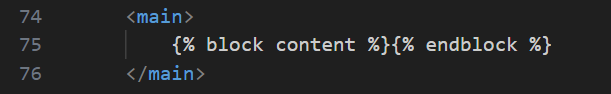
\includegraphics[width=1.0\textwidth]{base_blocks_example.png}
\end{figure}

Az 4.1. ábrán egy példa látható az oldal main részének a block-jára. Ezután, ha írni szeretnénk egy származtatott oldalon ebbe a block-ba, akkor a "content" nevű block-ba szánt kódot\verb|| és \verb|$| kód között kell megadnunk. Ennek hatására a származtatott oldalon megadott block kódot a base.html oldal main részébe fogja helyezni.

\begin{figure}[H]
	\caption{A navigációs sáv kódja}
	\label{fig:navigationbar}
	\centering
	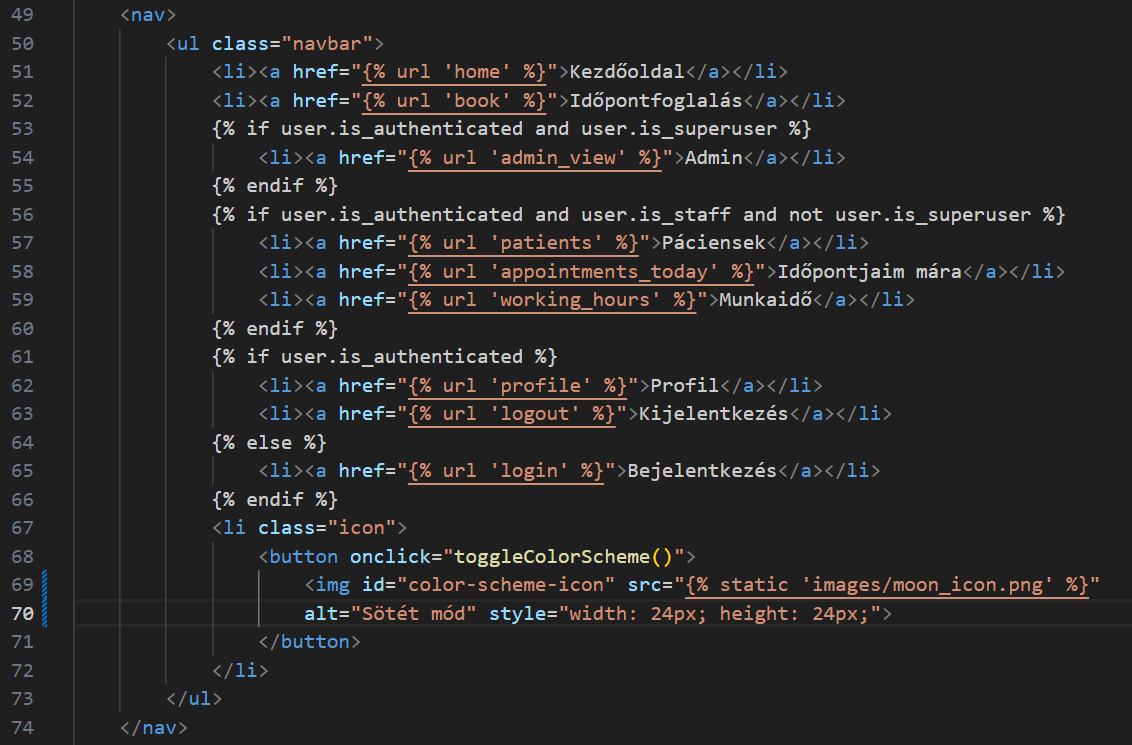
\includegraphics[width=1.0\textwidth]{navbar_code.png}
\end{figure}

A navigációs sáv kulcsfontosságú szerepet tölt be az alkalmazás felhasználhatóságában. A szakdolgozatomban az 4.2. ábrán látható módon oldottam meg a navigációs sáv implementációját a base.html fájlban. Az urls.py fájlban található linkeket adtam hozzá a Django sablonnyelvben írt feltételekkel, hogy a különböző jogokkal rendelkező felhasználók csak a nekik szánt oldalakat láthassák rajta. Ezek a linkek az alkalmazás tobábbi felhasználói felületeire navigálják a felasználót. Ezeken felül pedig van egy gomb is a navigációs sávon, ami a sötét, és világos módok közötti váltást teszi lehetővé egy JS kód segítségével, amire még a későbbiekben kitérek.



\chapter{User-szintű felhasználói felületek, és azok működése}
\label{chap:fejezet5}

A fogászati rendelő alkalmazás számos felülettel rendelkezik.

\section{A bejelentkezés és a regisztráció működése}

Az alkalmazásomban a regisztráció és bejelentkezés funkciók a Django beépített autentikációs rendszerére épülnek, amely lehetővé teszi a felhasználók kezelését, hitelesítését és jogosultságainak kezelését. Ez a funkció azért hasznos egy fejlesztőnek, mert ezáltal nem kell ezeket implementálnia minden új projektjébe.

\subsection{Az alkalmazás autentikációra használt metódusai:}

\begin{itemize}
	\item "authenticate": Ez a metódus ellenőrzi a felhasználó hitelesítő adatait (email és jelszó). Az EmailBackend osztály implementálja az "authentication.py" fájlban, és az email cím alapján keresi meg a felhasználót.
	\item "auth\_login": Bejelentkezteti a felhasználót, és a munkamenethez társítja. A Django beépített metódusa.
	\item "check\_password": Ellenőrzi, hogy a megadott jelszó megegyezik-e a titkosított jelszóval. A Django beépített metódusa.
	\item "set\_password": Beállítja az adott felhasználónak a jelszavát, és hashelt formában elmenti az adatbázisba. A Django beépített metódusa.
	\item "get\_user": Lekéri a felhasználót az azonosítója alapján. A Django beépített metódusa.
\end{itemize}

\begin{figure}[H]
	\caption{Az "authentication.py"}
	\label{fig:authentication}
	\centering
	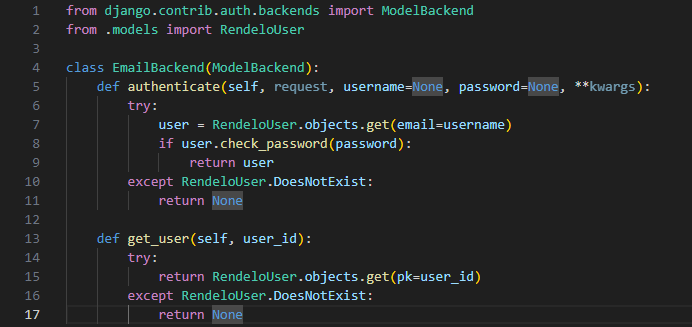
\includegraphics[width=1.0\textwidth]{authentication_py.png}
\end{figure}

\subsection{Regisztráció}

A regisztráció során a felhasználó a "register.html" fájlban megvalósított oldalon létrehozhat egy új fiókot, amelyet a rendszer a "RendeloUser" modellben tárol. A regisztrációs folyamat a következőképpen működik:

\begin{enumerate}
	\item Amikor a felhasználó megnyitja a regisztrációs oldalt, a "register\_view" nézet megjeleníti a regisztrációs űrlapot. Az űrlap két részből áll: a "RegistrationForm" a felhasználói fiók alapvető adatait (például felhasználónév, email cím, jelszó) kezeli, míg a "PatientForm" a páciens adatait (például név, születési dátum) tartalmazza.
	\item Az űrlap elküldése után a "register\_view" nézet ellenőrzi az űrlapok érvényességét. Ha az adatok helyesek, a "RegistrationForm" "save" metódusa létrehoz egy új RendeloUser példányt, amely a felhasználói fiókot reprezentálja. A jelszó titkosítva kerül tárolásra a "set\_password" metódus segítségével, ami az "AbstractUser" metódusa, amiből a "RendeloUser" osztály származik.
	\item A "PatientForm" létrehoz egy új Patient példányt, amely a páciens adatait tárolja. A "register\_view" nézet pedig beállítja a Patient $id$ adattagjának az értékét az újonnan létrehozott RendeloUser $id$ adattagjának az értékére, hogy a Patient példány azonosítója megegyezzen a RendeloUser példány azonosítójával, így a két objektum összekapcsolódhasson.
	\item A regisztráció sikeres befejezése után az "auth\_login" metódus automatikusan bejelentkezteti a felhasználót, és átirányítja a kezdőoldalra.
	\item A felhasználó beállított email címére egy email kerül kiküldésre, amelyben megköszöni a cég a regisztrációt. (Jelenleg egy konzolos email küldés van beállítva, csupán a demózás céljából.)
\end{enumerate}

\begin{figure}[H]
	\caption{A register\_view nézet}
	\label{fig:registerview}
	\centering
	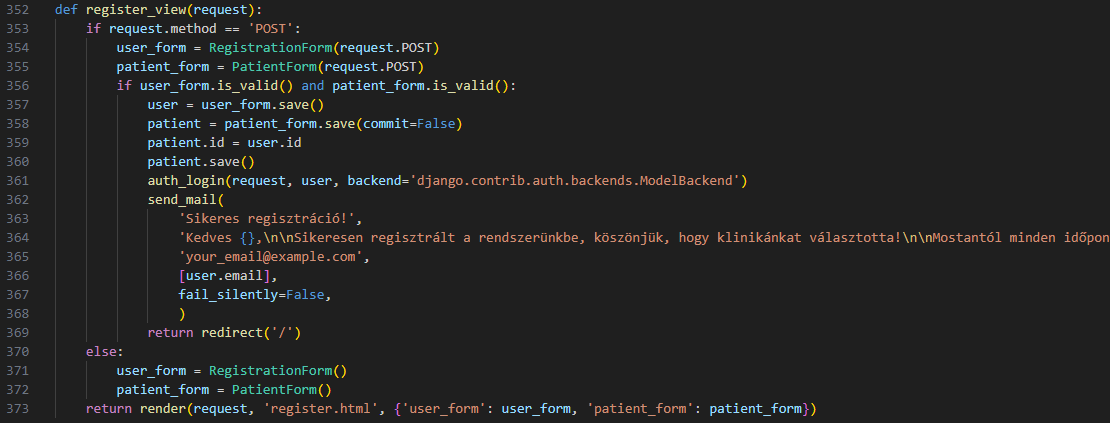
\includegraphics[width=1.0\textwidth]{register_view.png}
\end{figure}

\subsection{Bejelentkezés}

A bejelentkezés során a felhasználó a "login.html" fájlban megvalósított oldalon megadja az email címét és jelszavát, amelyek alapján a bejelentkezés történik. A folyamat a következőképpen működik:

\begin{enumerate}
	\item Amikor a felhasználó megnyitja a bejelentkezési oldalt, a "login\_view" nézet megjeleníti a bejelentkezési űrlapot. Az űrlap tartalmazza az email cím és jelszó mezőket.
	\item Az űrlap elküldése után a "login\_view" nézet az authentication.py "EmailBackend" osztályának "authenticate" metódusát hívja meg, amely az email cím és jelszó páros érvényességét ellenőrzi. Az "authenticate" metódus a "RendeloUser" modellben keresi meg a felhasználót az email cím alapján, majd a "check\_password" metódussal ellenőrzi a jelszót.
	\item Ha a hitelesítés sikeres, az "auth\_login" metódus bejelentkezteti a felhasználót, és a munkamenethez társítja. Ezután a felhasználó átirányításra kerül a kezdőoldalra.
	\item Ha a hitelesítés sikertelen (például helytelen email cím vagy jelszó miatt), a rendszer hibaüzenetet jelenít meg a felhasználónak.
\end{enumerate}

\section{A kezdőoldal}

Az összes szintű felhasználó bejelentkezés után a kezdőoldalon találja magát, amit a kezdooldal.html fájlban valósítottam meg. Az oldalon található a base.html elemein kívül egy marketing leírás a rendelőről, ami statikusan az oldalra van írva, nem lehet változtatni, csak a HTML kódban.
A leírás után pedig egy táblázat a rendelőben lehetséges kezelésekről, és azok árairól. A táblázat fejléce után Django sablon nyelven következik egy for ciklus, ami végigmegy az összes "Treatment" példányon az adatbázisban, és mindegyiknek a nevét, és az árát kiírja egy külön sorba. A Django Template fájlok az adatbázis objektumait a views.py egyik függvényétől kapják meg az 1.7. ábrán látható módon.

\begin{figure}[H]
	\caption{A kezdőoldal views.py-ban található megjelenítési függvénye}
	\label{fig:kezdooldal}
	\centering
	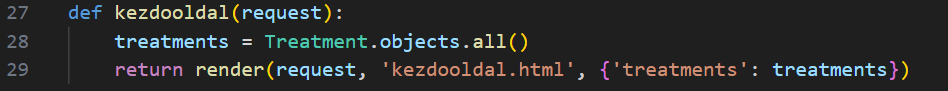
\includegraphics[width=1.0\textwidth]{kezdooldal_view.png}
\end{figure}

\section{Az időpontfoglalás}

Az időpontfoglalás oldal az egyik legösszetettebb része az alkalmazásnak. A foglalási folyamat során a felhasználó kiválasztja az orvost, a kezelést, a dátumot és az időpontot, majd a fizetési módot, ezzel elindítva az időpontfoglalás teljes folyamatát. A views.py fájlban definiált "idopontfoglalas" függvény koordinálja a folyamatot.

\subsection{Az időpontfoglalás lépései}
\begin{enumerate}
	\item Orvos kiválasztása:
	\begin{itemize}
		\item Interakció: A felhasználó az oldal tetején megjelenített orvosok listájából választ.
		\item Kód: JavaScript eseménykezelő aktiválódik, amely beállítja a "selected\_doctor" mező értékét a kiválasztott orvos azonosítójára, majd meghívja az "updateAvailableSlots()" függvényt.
	\end{itemize}
	\item Kezelés kiválasztása:
	\begin{itemize}
		\item Interakció: A felhasználó a legördülő menüből választja ki a kívánt kezelést.
		\item Kód: A kezelési opció módosítása szintén az "updateAvailableSlots()" függvényt indítja el, frissítve a kezeléshez tartozó időpontokat.
	\end{itemize}
	\item Dátum kiválasztása:
	\begin{itemize}
		\item Interakció: A felhasználó a naptármezőből választja ki a foglalni kívánt napot.
		\item Kód: A dátumválasztás után a JavaScript lekéri az adott napra vonatkozó szabad időpontokat az API végpontból, majd megjeleníti azokat.
	\end{itemize}
	\item Időpont kiválasztása:
	\begin{itemize}
		\item Interakció: A megjelenített időpontgombok közül a felhasználó kiválaszt egyet, vagy rákattint a "legközelebbi időpont" gombra.
		\item Kód: A kiválasztáskor a JavaScript beállítja az "appointment\_datetime" mező értékét (dátum és idő kombináció), illetve vizuálisan kiemeli a kiválasztott időpontot.
	\end{itemize}
	
	 Itt kihívásként említeném a felhasználó számára megjelenített elérhető időpontok megjelenítését. Azt kellett megoldanom, hogy ne csúszhassanak egymásba az időpontok. Tehát például ha le van foglalva valamilyen kezelésre egy időpont az adott dátumon 11:00-ra, akkor ne jeleníthessen meg a felhasználónak 10:45-re szabad időpontot, amikor egy 35 perc hosszúságú kezelést választott ki. Ezt az 5.4. ábrán látható metódussal oldottam meg, amit az "idopontfoglalas.html" JS kódja hív meg. A metódus először is 15-tel osztható számra kerekíti a kiválasztott kezelés hosszát felfelé, (például egy 50 perces kezelés hosszát 60 percesre kerekít), majd a HTML oldalon lévő JS kód által megjelenített időpontokat szűri. A get\_available\_slots metódus biztosítja, hogy csak azok az időpontok jelenjenek meg a felhasználónak, amelyek nem ütköznek más foglalásokkal. Ehhez a metódus minden egyes időintervallumot ellenőriz, hogy az adott időpontban és az azt követő időtartamban (a kezelés hossza alapján) ne legyen másik foglalás. A metódus figyelembe veszi az orvos munkaidejét is, így csak az orvos által megadott munkaidőn belüli időpontokat jeleníti meg. Az eredmény egy JSON válasz, amely tartalmazza az elérhető időpontokat és azok elérhetőségét. Ez a válasz a frontend JavaScript kódjában kerül feldolgozásra, amely a felhasználó számára vizuálisan is megjeleníti a szabad időpontokat.
	 
	  \begin{figure}[H]
	 	\caption{A get\_avaliable\_slots metódus implementációja a views.py-ban}
	 	\label{fig:getavaliableslots}
	 	\centering
	 	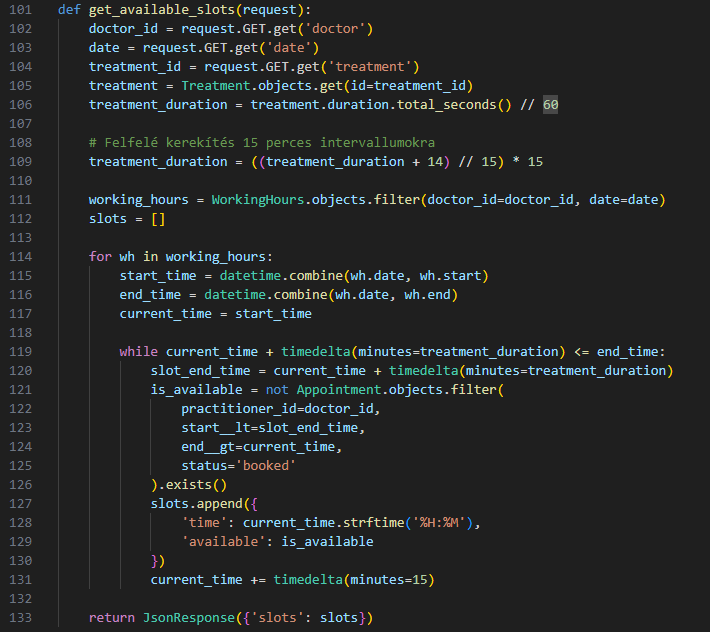
\includegraphics[width=1.0\textwidth]{get_avaliable_slots.png}
	 \end{figure}
	 
	 	\item Fizetési mód kiválasztása:
	 \begin{itemize}
	 	\item Interakció: A fizetési módok közül a felhasználó egyet választ (pl. online fizetés – PayPal vagy bankkártya, illetve helyszíni fizetés).
	 	\item Kód: A JavaScript eseménykezelő beállítja a "payment\_method" mezőt, amely később a Django backendben a foglalás véglegesítéséhez és a fizetési folyamat elindításához szükséges.
	 \end{itemize}
	 \item Foglalás véglegesítése:
	 \begin{itemize}
	 	\item Interakció: A felhasználó a „Foglalás” gombra kattint, miután minden kötelező adatot megadott.
	 	\item Kód: 
	 	\begin{itemize}
	 		\item A JavaScript egy megerősítő üzenetben összegzi a kiválasztott orvos, kezelés, dátum és időpont adatait.
	 		\item Ha a felhasználó megerősít, az űrlap elküldésre kerül, és a views.py "idopontfoglalas" függvénye végrehajtja az alábbiakat:
	 		\begin{itemize}
	 			\item Ellenőrzi az időpont elérhetőségét (szabad-e az adott időintervallum).
	 			\item Lekéri az orvos munkaidejét a WorkingHours modell alapján.
	 			\item Létrehoz egy új Appointment objektumot az adatbázisban.
	 			\item Rögzíti a foglalás fizetési státuszát a PaymentStatus modell segítségével.
	 			\item Ha a felhasználó online fizetést választott, átirányítja a fizetési oldalra a tranzakció elindításához.
	 		\end{itemize}
	 	\end{itemize}
	 \end{itemize}
\end{enumerate}


\begin{itemize}
	\item "updateAvailableSlots()" JavaScript függvény:
	Lekéri a kiválasztott orvos, kezelés és dátum alapján az elérhető időpontokat az API-ból, majd megjeleníti a délelőtti és délutáni időpontokat gombok formájában.
	\item "earliestAppointmentButton" eseménykezelő:
	A „Leghamarabbi időpont kiválasztása” gomb megnyomásakor az API-tól lekéri a legkorábbi szabad időpontot, majd automatikusan beállítja a dátumot és az időpontot.
	\item Űrlap beküldése:
	A foglalási űrlap beküldése előtt a JavaScript egy megerősítő párbeszédablakban összegzi a választott opciókat, majd a felhasználó jóváhagyása esetén elküldi az űrlapot. A Django view feldolgozza a POST kérést, létrehozza az időpontfoglalást, és ha a felhasználó az online fizetést választja, akkor a fizetési oldalra irányítja át, ha pedig a fizetés a helyszínen opciót, akkor a profil oldalra.
\end{itemize}

\section{A fizetési oldal}

A fizetési oldal a "payment\_page.html" oldalon lett megvalósítva. A fizetéshez a tématervembe OTP Simple Pay fizetési rendszert írtam, viszont egy kis kutatás után a PayPal-t könnyebben beépíthetőbbnek, stabilabbnak, és jobban átláthatóbbnak találtam. Ezért inkább azt építettem be az alkalmazásba.\\
A PayPal fizetés demózásához létre kellett hoznom egy sandbox PayPal fiókot, majd az azonosítómat használva importálnom kellett az oldalra egy JavaScriptet az alábbi módon: 

\begin{lstlisting}[caption={A PayPal sandbox importja},label={lst:stringstartswith}, language={HTML}]
<script src="https://www.paypal.com/sdk/js?client-id=Abw9kvI2SEa...&currency=HUF"></script>
\end{lstlisting}

Ezután egy "div"-hez hozzá kellett adnom a "paypal-button-container" id-t, és meg kellett valósítanom a fizetési logikát, amit az alábbi módon tettem meg a HTML fájlban:
 	
\begin{lstlisting}[caption={A fizetési logika},label={lst:stringstartswith}, language={HTML}]
	<script>
	paypal.Buttons({
		createOrder: function(data, actions) {
			return actions.order.create({
				purchase_units: [{
					amount: {
						value: '1', // Teszt osszeg
						currency_code: 'HUF'
					}
				}]
			});
		},
		onApprove: function(data, actions) {
			return actions.order.capture().then(function(details) {
				fetch("", {
					method: 'POST',
					headers: {
						'Content-Type': 'application/json',
						'X-CSRFToken': '{{ csrf_token }}'
					},
					body: JSON.stringify({
						orderID: data.orderID,
						status: details.status,
						orderRef: '{{ appointment.id }}'
					})
				}).then(response => {
					if (response.ok) {
						alert('A tranzakcio sikeresen megtortent: ' + details.payer.name.given_name);
						window.location.href = "";
					} else {
						alert('Hiba tortent a fizetes soran.');
					}
				}).catch(error => {
					console.error('Hiba tortent a fizetes soran:', error);
					alert('Hiba tortent a fizetes soran.');
				});
			});
		},
		onError: function(err) {
			console.error(err);
			alert('Hiba tortent a fizetes soran.');
		}
	}).render('#paypal-button-container');
	</script>
	
\end{lstlisting}

Ennek hatására a fizetési oldalon egy bankkártya, vagy egy PayPal fiókos fizetési opció jelenik meg, amiből a felhasználó tud választani. Ha a fizetés sikeres, akkor az időponthoz tartozó "PaymentStatus"-nak az $is\_paid$ adattagját "true"-ra állítja, és a felhasználót átirányítja a Profil oldalra, ahol a lefoglalt időpontnál látszik a "Fizetve" felirat. Ha nem sikerült a fizetés akkor kiírja a hibaüzenetet, és nem állítja az $is\_paid$ adattagot "true"-ra.

\section{A profil oldal}

A profil oldal mindhárom felhasználói jogosultságú felhasználó számára látható, viszont mindhárom típusú felhasználó számára más jelenik meg rajta. A "ProfileForm" mindenképp megjelenik, ezen tudja változtatni a felhasználó a felhasználónevét, az email címét, és a jelszavát. Ez a form szerkeszti a "RendeloUser" modellt. A "profile\_view" metódus a views.py fájlban az 5.5. ábrán látható módon vizsgálja meg a felhasználó jogosultságát, hogy ez alapján jelenítse meg a formokat a felhasználó számára. Ha a felhasználó "superuser", akkor semmit nem jelenít meg a "ProfileForm" után (a $patient\_form$ változó amúgy is none kezdőértékű), ha nem "superuser", hanem "staff", akkor ez azt jelenti, hogy egy orvos kattintott az oldalra, tehát lekéri azt a "Doctor" osztálypéldányt az adatbázisból, amelyiknek egyezik az azonosítója a bejelentkezett felhasználó azonosítójával, és a $doctor\_form$ változóba is lekéri az adott formot, és átadja neki a "Doctor" példányt, amit lekért. Ha pedig nem is "staff" a felhasználó, akkor a "Patient" példányt és formot kéri le hozzá.

\begin{figure}[H]
	\caption{A profile\_view metódus form kiválasztása}
	\label{fig:profileviewformkivalasztas}
	\centering
	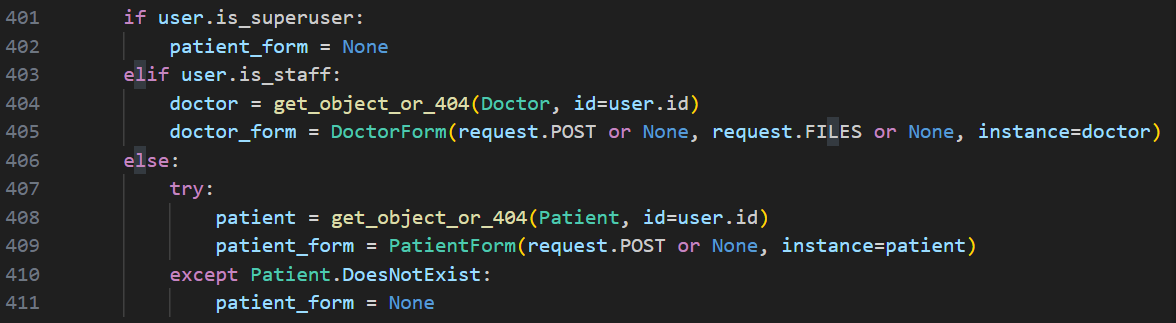
\includegraphics[width=1.0\textwidth]{profile_view_forms.png}
\end{figure}

A formok kitöltve jelennek meg a felhasználók adataival az oldalon, amiket változtathatnak és a formok után található "Mentés" gombbal a változtatásaik elmenthetők.

"User" szintű felhasználó esetében megjelennek a formok után a felhasználó által lefoglalt időpontok is, dátum szerint csökkenő sorrendben. Az időpontok kattinthatók, ezek átvisznek az "edit\_appointment.html" "read only" nézetébe, ahol a felhasználó megtekintheti az adott időponthoz írt kezelés leírást, és az időpont adatait bővebben. Például hogy fizetve van-e, vagy hogy melyik orvoshoz lett foglalva. Az időpontok le is mondhatók a "Lemondás" gombbal a profil oldalon abban az esetben, ha dátum szerint legalább egy nappal későbbre lettek lefoglalva. Az időpont lemondásához megerősítést kér az oldal egy párbeszédablakban. Az időpont törlését a views.py fájlban található "cancel\_appointment" metódus végzi.

\chapter{Staff-szintű felhasználói felületek, és azok működése}
\label{chap:fejezet6}

Ahogy a korábbiakban már leírtam, az alkalmazásban a Staff felhasználói szint az orvosokat reprezentálja. Nekik lehetőségük van belenézni bármelyik páciens kezeléstörténetébe, és hozzáférnek a páciensek elérhetőségéhez is. Továbbá megadhatják a saját munkaidejüket, és megnézhetik a saját időpontjaikat dátumonként szűrve. Ugyanakkor időpontfoglaláshoz nincs joguk, nem is lenne lehetséges, mivel az orvosok fiókjaihoz nincs "Patient" példány rendelve.

\section{A "Páciensek" oldal}

Ezen az oldalon az orvos rákereshet bármelyik páciensre név szerint az oldalon lévő kereső segítségével, vagy az "Összes páciens" gombra kattintva visszatérhet az alapértelmezett nézetbe, ami az összes adatbázisban lévő pácienst kilistázza az oldalon látható táblázatba. Az oldal a "patients.html" fájlban lett megvalósítva. Mindegyik páciens kattintható, kattintás hatására az adott páciens adatlapjára jut a felhasználó, ami a "patient.html" oldalon lett megvalósítva. Ezen az oldalon vannak a páciensnek az adatai láthatók amelyikre a felhasználó kattintott, továbbá az összes lefoglalt időpontja és azoknak leírása időrend szerint csökkenő sorrendben. Az oldalon alapértelmezetten minden a páciens által lefoglalt időpont megjelenik, viszont a felhasználónak lehetősége van hónap alapján szűrni őket, ezzel könnyebbé téve a kezeléstörténet vizsgálatát. Az oldalon található még egy "Vissza a páciensekhez" gomb, ami visszavezet a "Páciensek" oldalra. A 6.1. ábrán ennek az oldalnak a kinézete látható.

\begin{figure}[H]
	\caption{A "Páciensek" oldal}
	\label{fig:paciensek}
	\centering
	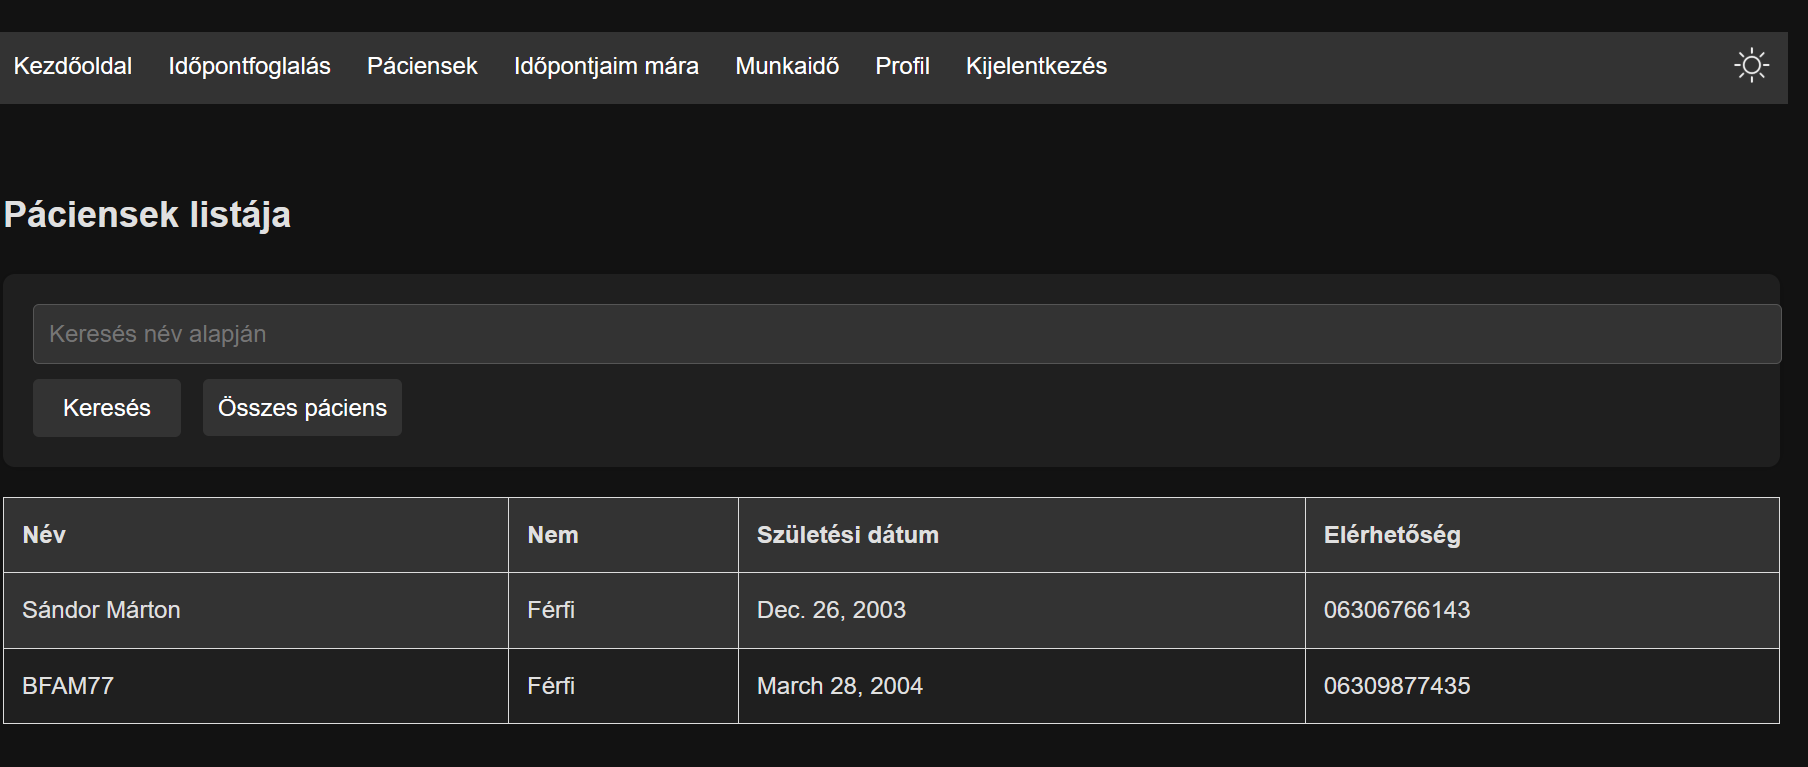
\includegraphics[width=1.0\textwidth]{patients_page.png}
\end{figure}

\section{Az "Időpontjaim mára" oldal}

Ezen az oldalon láthatja az orvos a hozzá foglalt időpontokat a megadott dátumon.

\begin{figure}[H]
	\caption{Az "Időpontjaim mára" oldal}
	\label{fig:idopontjaimmara}
	\centering
	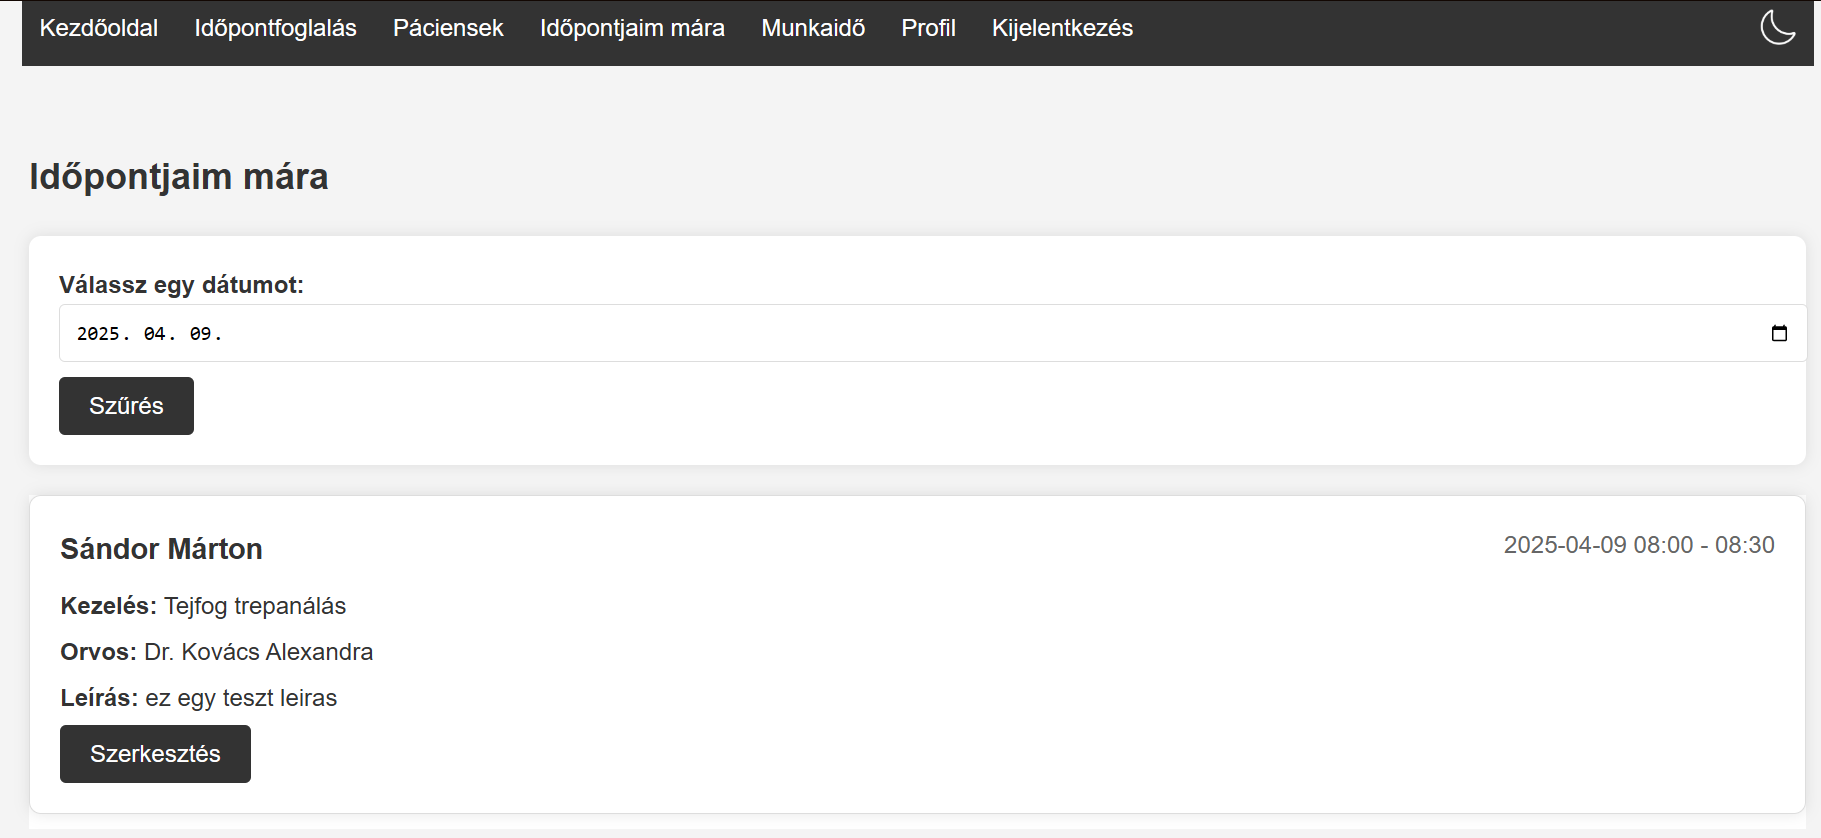
\includegraphics[width=1.0\textwidth]{idopontok_mara.png}
\end{figure}

A 6.2. ábrán látható módon jelennek meg az időpontok az oldalon. Alapértelmezetten a jelenlegi dátumra lefoglalt időpontok jelennek meg, viszont a beviteli mező segítségével a más dátumokra foglalt időpontokat is meg lehet nézni. Egy adott időpontnál a "Szerkesztés" gomb átnavigálja a felhasználót az "Időpont adatai" oldalra, ahol a "user" típusú felhasználók csak nézhetik az időpontjaik adatait, viszont az orvosoknak lehetőségük van szerkeszteni azok leírását. Így adható meg a páciens kezeléstörténete. Ez az oldal az "edit\_appointment.html" oldalon lett megvalósítva.

\begin{figure}[H]
	\caption{Az "Időpont adatai" oldal}
	\label{fig:idopontadatai}
	\centering
	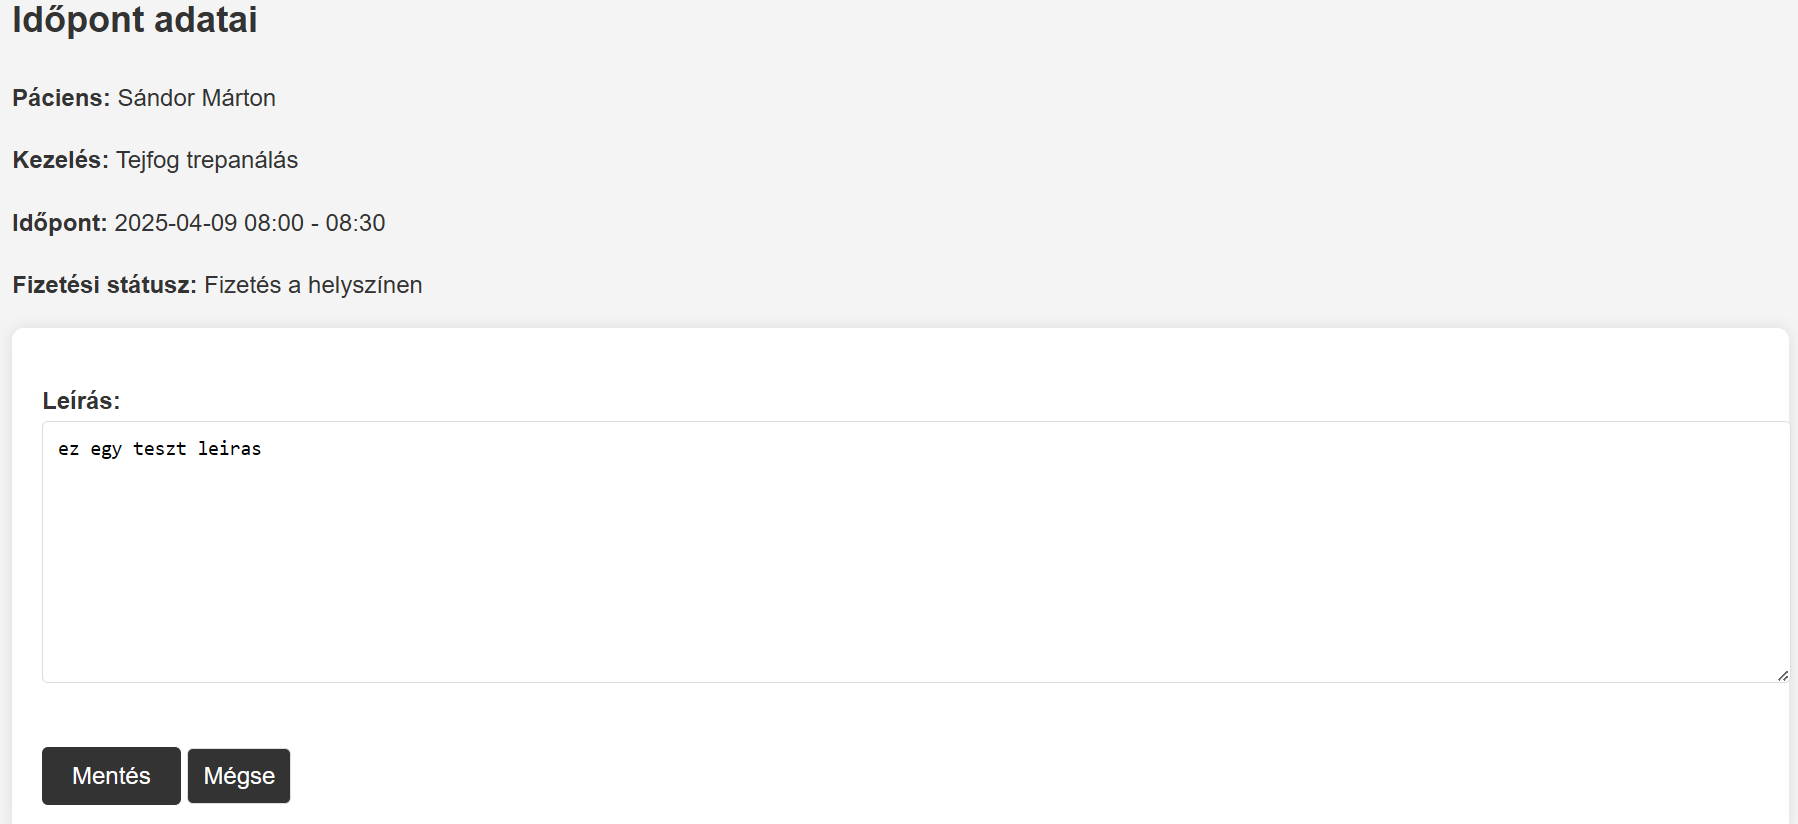
\includegraphics[width=1.0\textwidth]{idopont_szerkesztes.png}
\end{figure}

A "Metés" gombbal elmenthető a leírás amit az időponthoz rendeltünk, a "Mégse" gomb pedig visszanavigál az "Időpontjaim mára" oldalra.

\section{A "Munkaidő oldal"}

Az orvos a munkaidejét ezen az oldalon állíthatja be. Az oldal a "working\_hours.html" fájlban lett megvalósítva.

\begin{figure}[H]
	\caption{A munkaidő megadása}
	\label{fig:munkaidomegadasa}
	\centering
	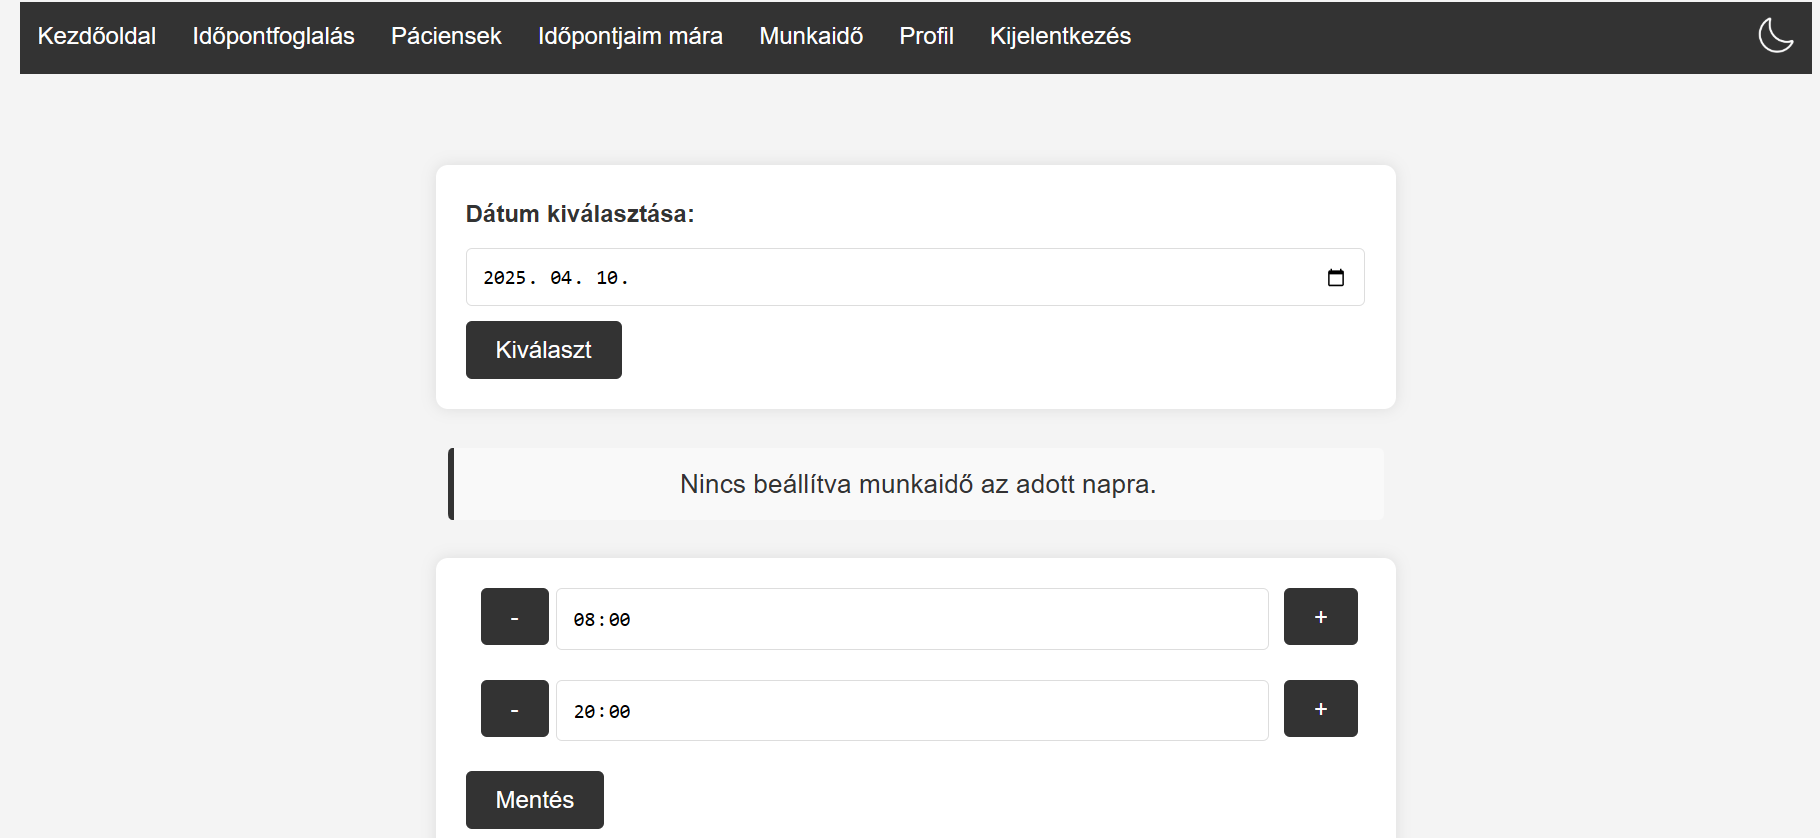
\includegraphics[width=1.0\textwidth]{working_hours.png}
\end{figure}

Amikor a felhasználó ellátogat az oldalra és kiválaszt egy dátumot, akkor a 6.4. ábrán látható kép fogadja. A rendelő 8:00-20:00 között van nyitva, tehát ennél korábbi kezdést, vagy későbbi végzést nem lehet beállítani munkaidőnek. A kezdés és végzés ideje a + és - gombokkal növelhető, vagy csökkenthető. Egy kattintás 15 perccel növeli, vagy csökkenti a beviteli mezőben látható időt. A beviteli mező ezeken a gombokon kívül mással nem szerkeszthető. Ez azért van, hogy a felhasználó ne adhasson meg magának olyan kezdési, vagy végzési időpontot, ami nem "kerek", és az időpontfoglalási rendszert összezavarná. A munkaidőt beállítani, vagy a már beállítottat szerkeszteni a "Mentés" gombbal lehet. Ennek a hatására az alkalmazás elmenti a "WorkingHours" modellbe az orvos munkaidejét. Abban az esetben, ha még a kiválasztott napra nincs megadva az adott orvosnak munkaidő, akkor megjelenik a képen látható üzenet is az oldalon.

\section{Az orvosok Profil oldala}

Az orvosok profil oldala ugyan abban a fájlban lett megvalósítva ugyan azzal a működési elvvel, mint az az oldal, amit az 5.5. fejezetben bemutattam. Azonban ennél a típusú felhasználónál akadtak nehézségek, mivel a "DoctorForm" form töltődik be a "PatientForm" helyett, és ennek a formnak kezelnie kell képeket. Itt is a Django beépített fájlbeviteli mezőjét szerettem volna használni, de azt nem sikerült CSS kóddal designolnom, és nem nyújtott kellően szép látványt. A megoldásom az lett erre a problémára, hogy készítettem egy saját képbeviteli oldalt a "custom\_clearable\_file\_input.html" fájlba, készítettem a "forms.py"-ba egy osztályt hozzá, és a 6.5. ábrán látható módon beleraktam a "DoctorForm"-ba, hogy ezt használja a képek beviteléhez.

\begin{figure}[H]
	\caption{A "DoctorForm"}
	\label{fig:doctorform}
	\centering
	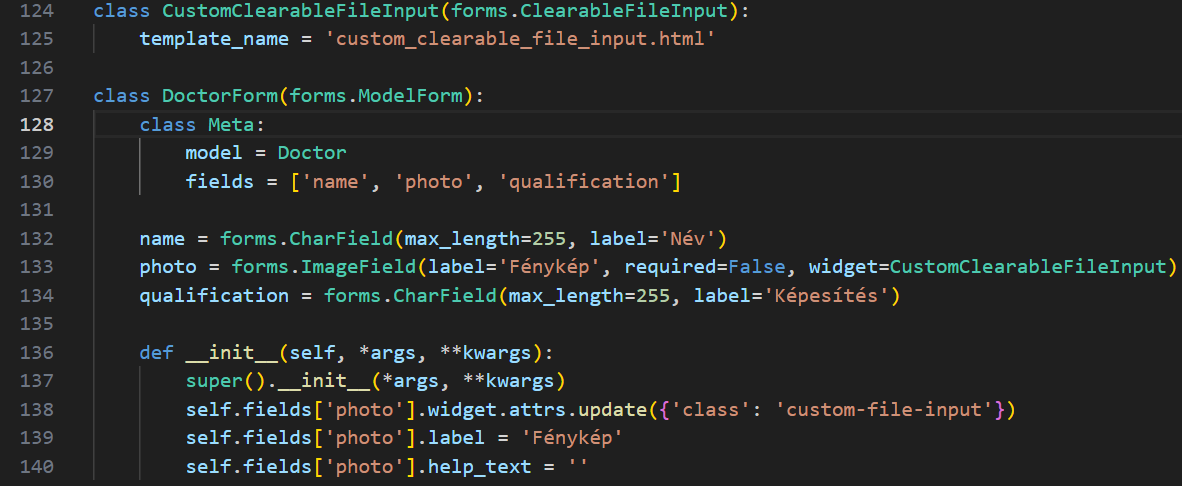
\includegraphics[width=1.0\textwidth]{doctor_form.png}
\end{figure}

Ezt már lehetett CSS kóddal designolni, így megoldódott a probléma, és a 6.6. ábrán látható is a munka eredménye.

\begin{figure}[H]
	\caption{A "DoctorForm" megjelenítése}
	\label{fig:doctorformview}
	\centering
	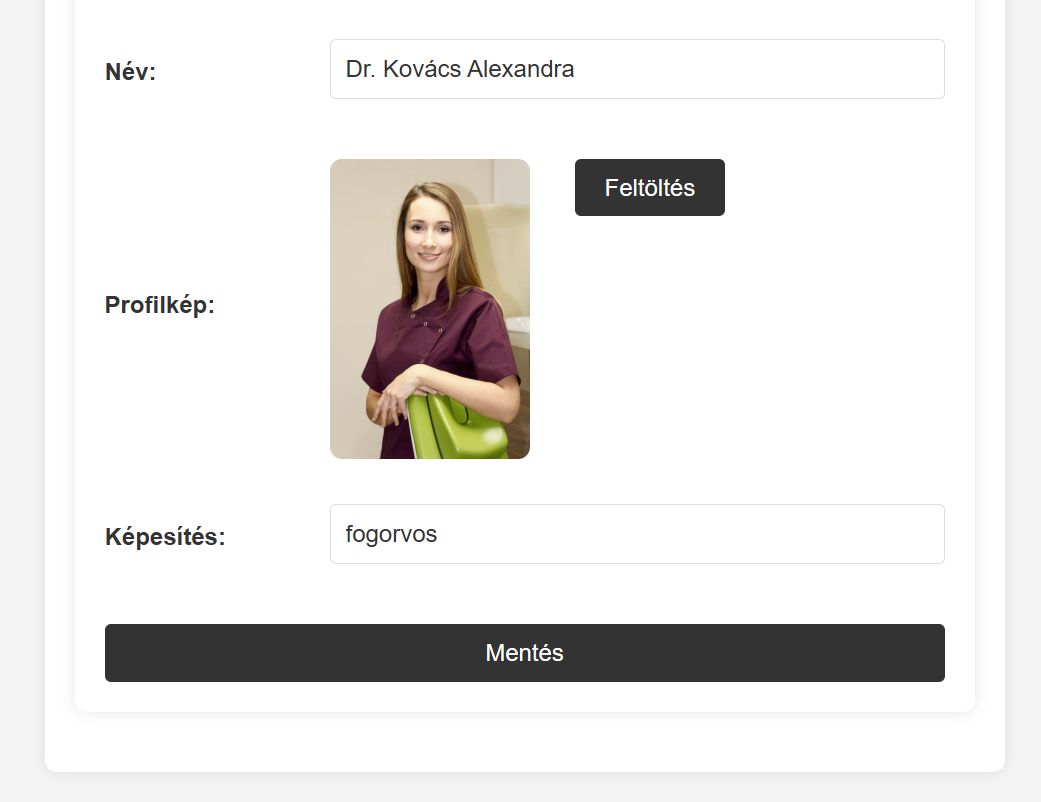
\includegraphics[width=1.0\textwidth]{doctor_form_view.png}
\end{figure}

A "Feltöltés" gomb megnyomásával ki lehet választani a képet, amit a felhasználó profilképként szeretne használni. Ez a kép jelenik meg a pácienseknek az időpont foglalásnál is, amikor az orvos kiválasztására kerül sor. A program a profilképeket a rendelo/media/doctor\_pictures mappába menti.




\chapter{Superuser-szintű felhasználói felületek, és azok működése}
\label{chap:fejezet7}

A Superuser szintű felhasználók az oldal adminisztrátorai. Nem tartozik a profiljukhoz sem "Patient" példány, sem "Doctor" példány. A felhasználók személyes adatain kívül mindenhez hozzáférnek az adatbázisban, és mindent joguk van törölni, vagy módosítani. A Django beépített admin felületére is van joguk bejelentkezni. Időpontot foglalni viszont nem tudnak, hasonló okok miatt, mint az orvosok.

\section{Az "Admin" oldal}

Az Admin oldal az "admin.html" fájlban lett megvalósítva, az adminisztrátor ezen az oldalon éri el az összes admin felületet.

\begin{figure}[H]
	\caption{Az "Admin" oldal}
	\label{fig:adminpage}
	\centering
	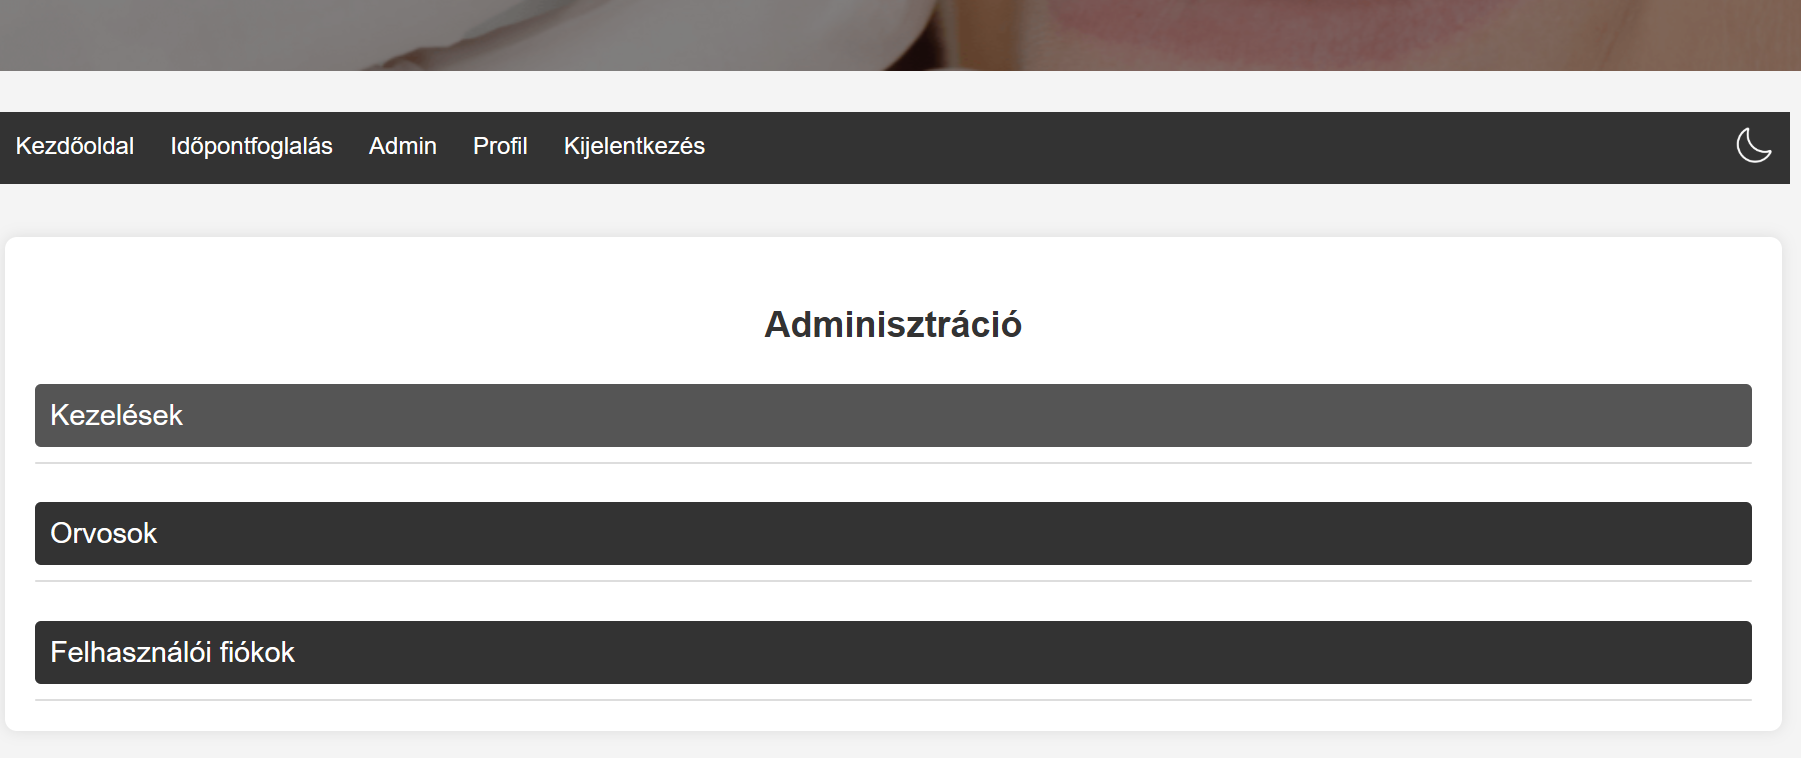
\includegraphics[width=1.0\textwidth]{admin_page.png}
\end{figure}

Az oldalon a 7.1. ábrán látható három lenyíló menü fogadja a felhasználót. Ezekben vannak a kezelések, az orvosok, és a felhasználói fiókok szerkesztési lehetőségei.

Ha lenyitja a kezeléseket akkor kilistázza az oldal az adatbázisban található összes megadott kezelést. A lenyíló gomb alatt található egy "Új kezelés hozzáadása" gomb, ami az "add\_treatment.html" oldalra navigálja a felhasználót. Ezen az oldalon a "TreatmentForm" található, amiben megadhatja a hozzáadni kívánt kezelés adatait, majd a "Mentés" gombbal elmentheti, vagy a "Mégsem" gombbal visszatérhet az Admin oldalra.

A kilistázott kezeléseknél mindegyikhez jut két gomb: "Törlés", vagy "Szerkesztés".

A "Törlés" a "Delete\_treatment.html" fájlba navigálja a felhasználót, ahol megkérdezi az oldal, hogy biztosan törölni kívánja-e a kezelést, és megjeleníti a kezelés adatait is. Az oldalon található "Törlés" gomb értelem szerűen törli, míg a "Mégsem" gomb visszanavigál az Admin oldalra.

A "Szerkesztés" gomb az "edit\_treatment.html" oldalra navigál, ahol szintén megjelenik a "TreatmentForm" a kiválasztott kezelés adataival kitöltve. Bármilyen adatot átírhat itt is a felhasználó, az oldalon lévő "Mentés" és "Mégsem" gombok pedig a megszokott módon működnek.

Az orvosok lenyíló menüben is hasonló lehetőségek találhatók, kilistázza az oldal az összes adatbázisban szereplő orvost egymás alá, és lehet újat elmenteni, szerkeszteni, és törölni az adatbázisból. Az új hozzáadása és a szerkesztés a "ProfileForm", és "DoctorForm" egítségével történik. Ezekhez a műveletekhez is külön oldalakat készítettem az alábbi fájlokban:

\begin{itemize}
	\item "add\_doctor.html"
	\item "edit\_doctor.html"
	\item "delete\_doctor.html"
\end{itemize}

Fontos, hogy itt az új orvos hozzáadása nem csak egy új "Doctor" példányt ad hozzá az adatbázishoz, hanem először létrehoz egy "RendeloUser"-t is, és annak az $id$-jával hozza létre a "Doctor"-t, hogy az orvos azonnal használhassa a felhasználói fiókját is. Az új orvos létrehozása esetén az orvos a megadott email címére meg is kap egy emailt, amiben megkapja a belépési adatait, hogy meg tudja őket változtatni.

A felhasználói fiókok lenyíló menüben ismét az adatbázisban található összes adat fogadja a felhasználót kilistázva, viszont ezeket lehetősége van szűrni a megszokott módon felhasználónév alapján.

\begin{figure}[H]
	\caption{Felhasználói fiókok}
	\label{fig:felhasznaloifiokok}
	\centering
	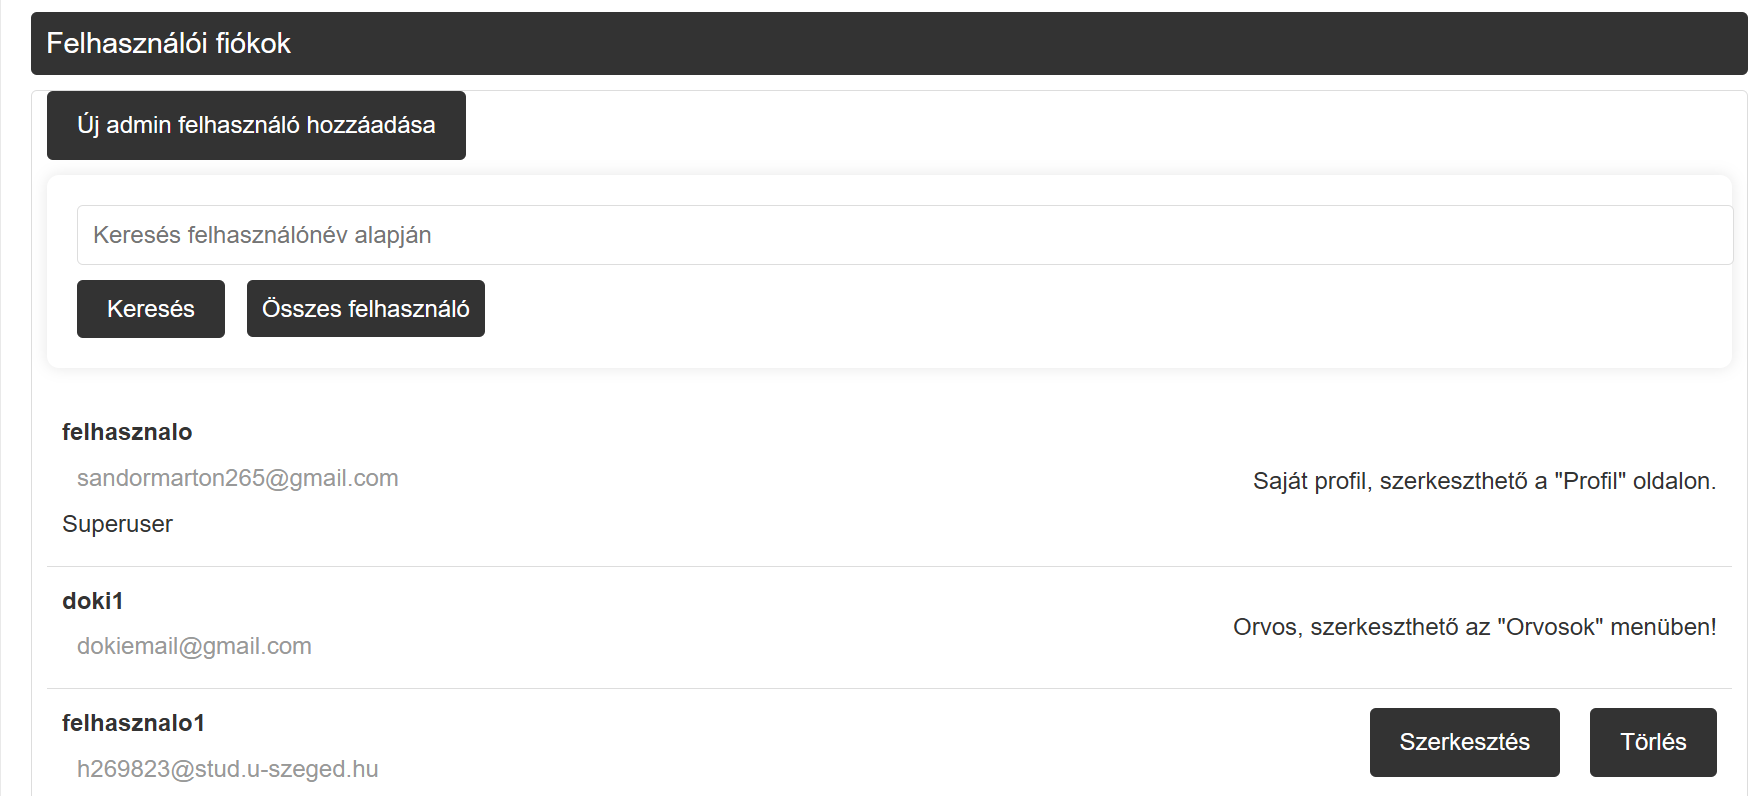
\includegraphics[width=1.0\textwidth]{admin_page_felhasznaloi_fiokok.png}
\end{figure}

Az adminisztrátornak joga van új admin felhasználót hozzáadnia az adatbázishoz, amit az "Új admin felhasználó hozzáadása" gombbal tehet meg. Ez elvezeti az "add\_admin\_user.html" oldalra, amin a "CustomUserCreationForm" segítségével a megszokott módon létrehozhat új rekordot az adatbázisba.

A kilistázott felhasználók közül itt nem szerkeszthetők az orvosok, mivel azokhoz ott van az orvosok szerkesztési oldala, és itt nem szerkeszthető, vagy törölhető az admin saját fiókja sem. Ez egy védelem, hogy az alkalmazás ne maradhasson adminisztrátor nélkül. A szerkesztést viszont meg tudja oldani a saját "Profil" oldalán, ami ugyan úgy működik, mint a többi szintű felhasználó esetében.

A "user" szintű felhasználókat, és a többi adminisztrátort pedig ugyan úgy tudja szerkeszteni a "ProfileForm", és a "PatientForm" segítségével, vagy törölni a megszokott módon. Ezekhez is készítettem két külön oldalt:

\begin{itemize}
	\item "edit\_user.html"
	\item "delete\_user.html"
\end{itemize}

\chapter{Design}
\label{chap:fejezet8}

A Design-t összesen 3 CSS fájllal oldottam meg. Ezek a fájlok a rendelo/static/Css mappában találhatók:

\begin{itemize}
	\item style.css: Az oldalak kinézetét írtam meg benne színek nélkül.
	\item colors\_light.css: Az alkalmazás világos módjának a színbeállításait írtam meg benne.
	\item colors\_dark.css: Az alkalmazás világos módjának a színbeállításait írtam meg benne.
\end{itemize}

\begin{figure}[!htbp]
	\caption{A "base.html" kinézete, és a navbar világos módban}
	\label{fig:lightmode}
	\centering
	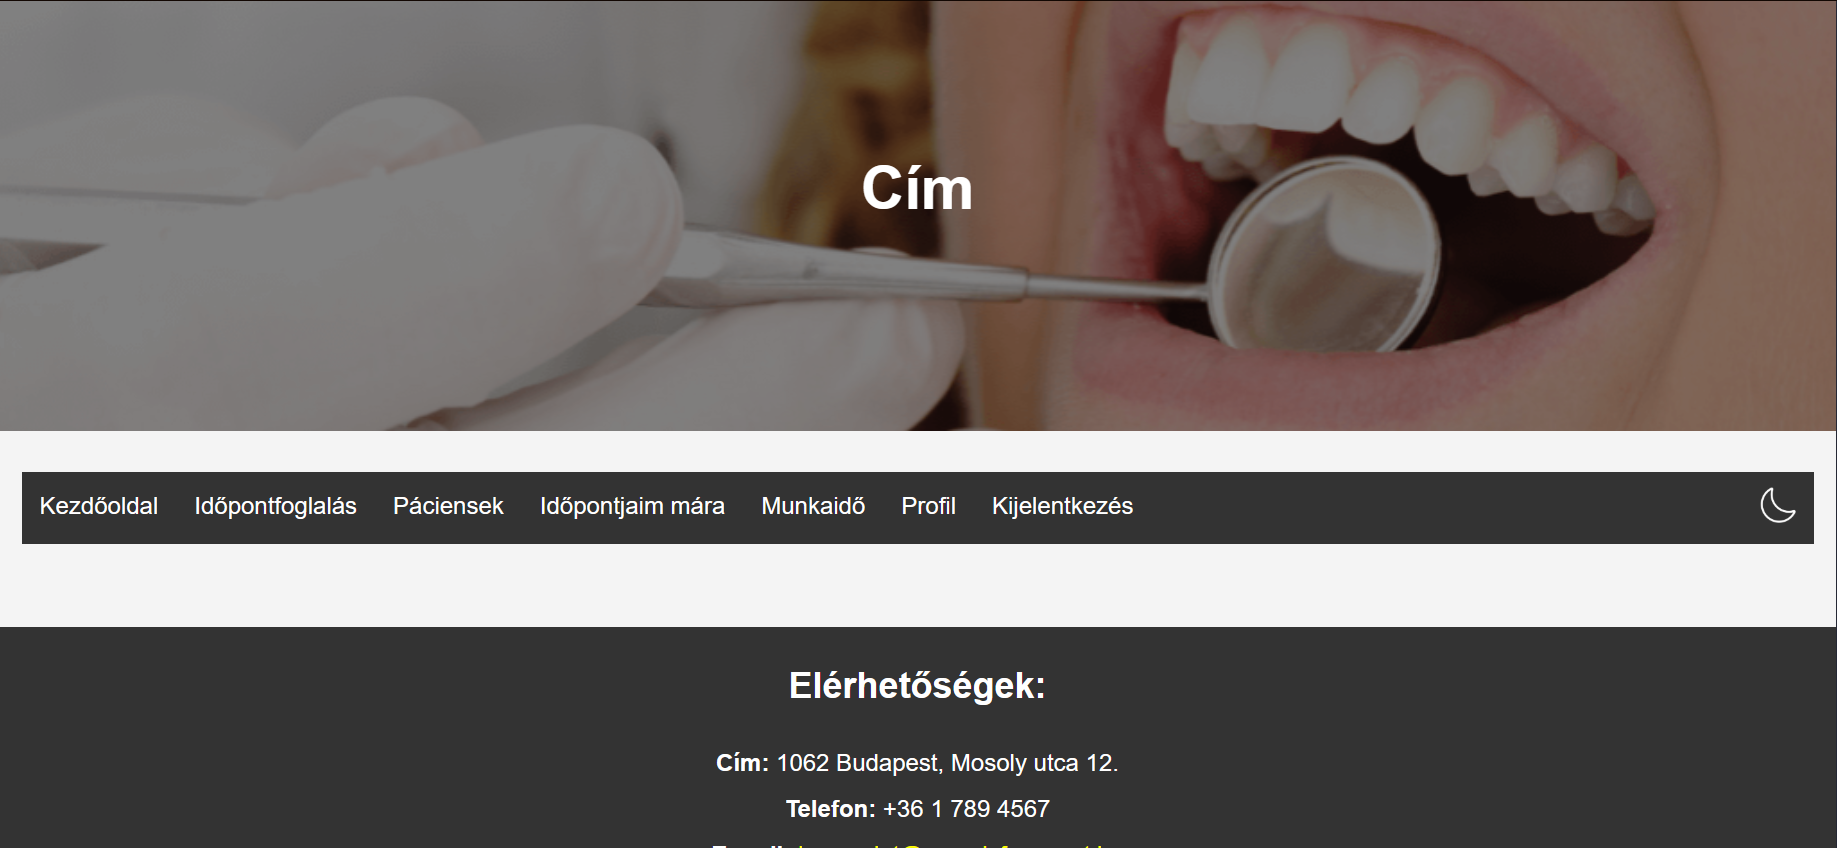
\includegraphics[width=1.0\textwidth]{base_page_light.png}
\end{figure}

A 8.1. ábrán világos módban megtekinthető a "base.html". Ahogy korábban már írtam, ebből származik az összes többi oldal, így mindegyik ezt a designt követi. Sötét módba a navigációs sáv jobb oldalán lévő "hold" ikonnal léphetünk.

\begin{figure}[!htbp]
	\caption{A "base.html" kinézete, és a navbar sötét módban}
	\label{fig:darkmode}
	\centering
	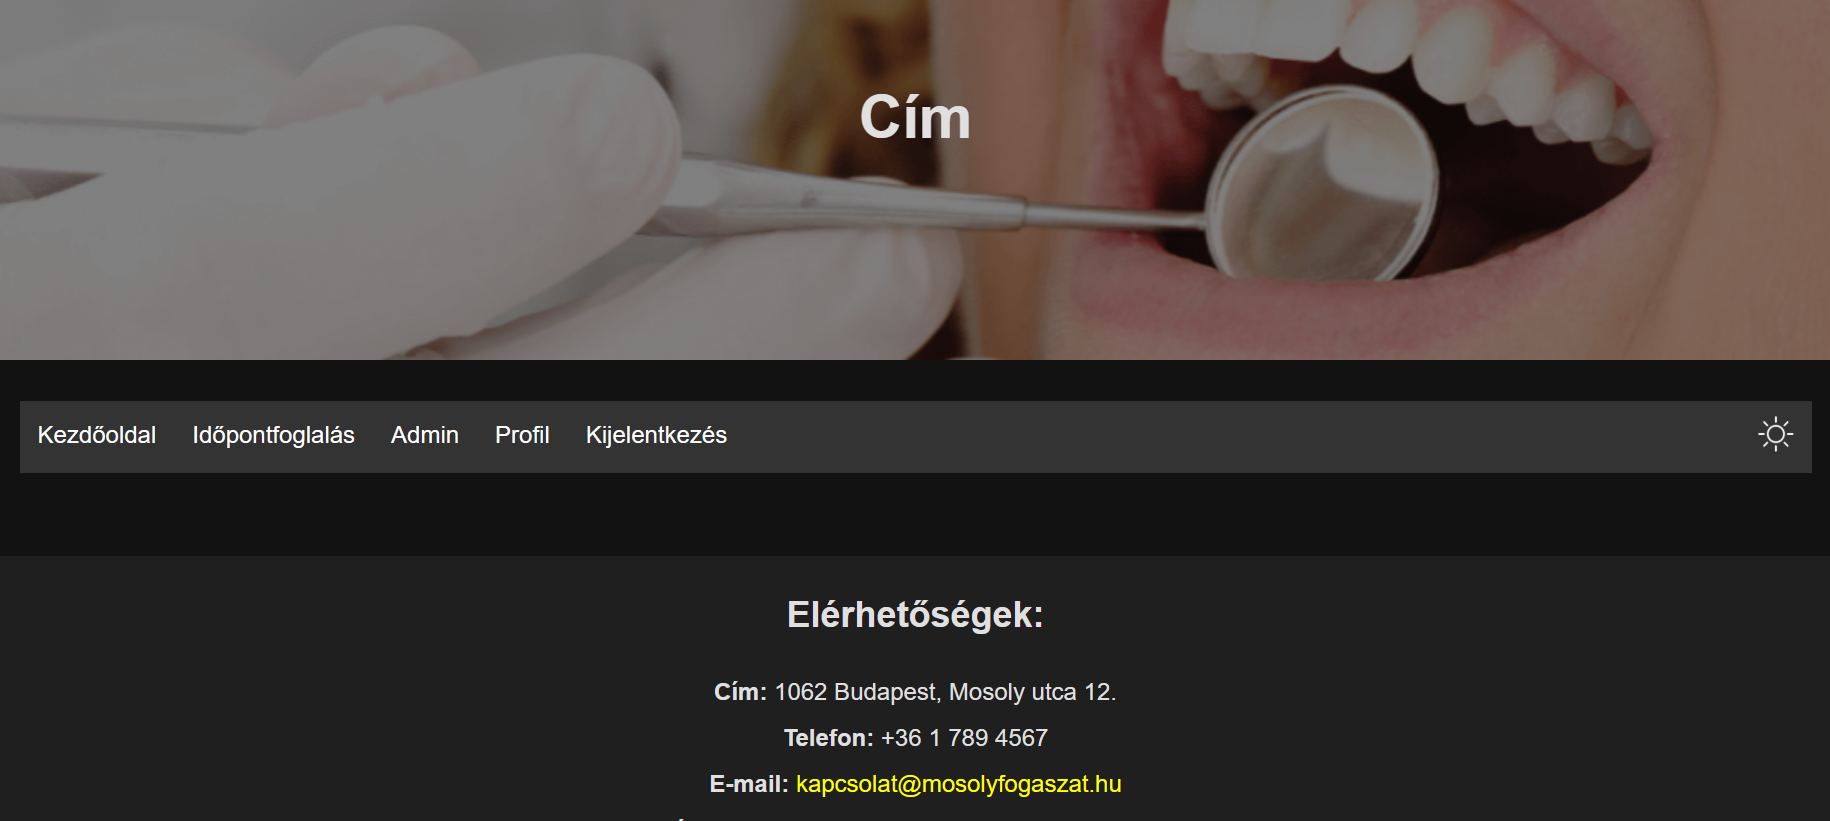
\includegraphics[width=1.0\textwidth]{base_page_dark.png}
\end{figure}

Ezt a "base.html" fájlban megírt JS kód hajtja végre:

\begin{lstlisting}[caption={A színösszeállítások között váltó JS kód},label={lst:stringstartswith2}, language={HTML}]
	<script>
	function toggleColorScheme() {
		const currentScheme = document.getElementById('color-scheme').getAttribute('href');
		const newScheme = currentScheme.includes('colors_light.css') ? 'colors_dark.css' : 'colors_light.css';
		document.getElementById('color-scheme').setAttribute('href', `` + newScheme);
		localStorage.setItem('color-scheme', newScheme);
		updateIcon(newScheme);
	}
	
	function updateIcon(scheme) {
		const icon = document.getElementById('color-scheme-icon');
		if (scheme.includes('colors_light.css')) {
			icon.src = '';
			icon.alt = 'Sotet mod';
		} else {
			icon.src = '';
			icon.alt = 'Vilagos mod';
		}
	}
	
	document.addEventListener('DOMContentLoaded', function() {
		const savedScheme = localStorage.getItem('color-scheme') || 'colors_light.css';
		document.getElementById('color-scheme').setAttribute('href', `` + savedScheme);
		updateIcon(savedScheme);
	});
	</script>
	
\end{lstlisting}

Alapértelmezetten a világos mód Css fájlját improtálja, viszont ha kattintunk a "hold" ikonra, akkor átírja az importot a sötét mód Css fájljának az importjára, majd utána átváltja "napra" az ikont, amire kattintottunk jelezve ezzel, hogy az a világos módba vezet. A design megírásához sima Css-t használtam.


\chapter{Összefoglaló}
\label{chap:conclusion}

\lipsum[50-53]
\chapter*{Nyilatkozat}
\addcontentsline{toc}{section}{Nyilatkozat}

% A szövegben a dolgozat típusa alapján "diplomamunkámat" vagy "szakdolgozatomat"
% szövegrészt készíti el. 
\ifthenelse{\equal{\dolgozatTipusa}{Diplomamunka}}
  {% True case
   \newcommand{\dolgozatomat}{diplomamunkámat}%
  }
  {% false case
   \newcommand{\dolgozatomat}{szakdolgozatomat}%
  }
%

\noindent Alulírott \nev{} \szak{} szakos hallgató, kijelentem, hogy a dolgozatomat a Szegedi Tudományegyetem, Informatikai Intézet \tanszek{} Tanszékén készítettem, \szak{} diploma megszerzése érdekében. 

Kijelentem, hogy a dolgozatot más szakon korábban nem védtem meg, saját munkám eredménye, és csak a hivatkozott forrásokat (szakirodalom, eszközök, stb.) használtam fel. 

Tudomásul veszem, hogy \dolgozatomat{} a Szegedi Tudományegyetem Informatikai Intézet könyvtárában, a helyben olvasható könyvek között helyezik el.

\vspace*{2cm}

\begin{table}[!h]
  \begin{tabular}{lc}
    Szeged, \vegsoDatum{} \hspace{2cm}  & \makebox[7cm]{\dotfill} \\
                                        & aláírás \\
  \end{tabular}
\end{table}

\thispagestyle{plain}
\addcontentsline{toc}{chapter}{Irodalomjegyzék}
\bibliographystyle{plain}
\bibliography{references}

\end{document}
